%!TEX root = ..\ms-thesis.tex
\chapter{Results and Discussion} \label{ch:results-discussion}

\section{Hot Ductility Curves}
The on-heating and on-cooling hot ductility curves for the Cone~1 and Cone~5 materials are presented in Figure~\ref{fig:c1-hot-ductility} and Figure~\ref{fig:c5-hot-ductility} respectively.  In general, the on-heating ductility for both Cones increased with testing temperature, up to a ductility maximum, before dropping rapidly to zero over a short temperature range.  From Figure~\ref{fig:c1-hot-ductility} and Figure~\ref{fig:c5-hot-ductility}, it is apparent that Cone~1 and Cone~5 also showed similar trends in on-cooling behavior, in that the on-cooling ductility remains essentially zero for a definite temperature range below the \gls{ndt} before gradually increasing at lower test temperatures.  Specifically for Cone~1, it is apparent from Figure~\ref{fig:c1-hot-ductility} that the Cone~1 material exhibited an on-heating \gls{ndt} of 2375\textdegree{}F and an on-cooling \gls{drt} of 2300\textdegree{}F, resulting in a \gls{ndr} of 75F\textdegree{}.  Figure~\ref{fig:c5-hot-ductility} shows that the Cone~5 material also exhibited an on-heating \gls{ndt} of 2375\textdegree{}F, \gls{drt} of 2300\textdegree{}F, and \gls{ndr} of 75F\textdegree{}.  These characteristics of the hot ductility curves for both materials are summarized in Table~\ref{tab:hot-ductility-results}.

\begin{figure}[h!]
    \setlength{\abovecaptionskip}{15pt}
    \centering
    \includegraphics[width=6in]{figures/hot-ductility/c1-hot-ductility-curve.pdf}
    \caption[Hot Ductility Behavior of Cone~1 Base Metal.]{Hot Ductility Behavior of CT15C Cone~1 Base Metal.  Bars indicate range of \%RA values at indicated test temperature.  On-Heating Curve Exhibits Class H1 behavior with \gls{ndt} = 2375\textdegree{}F; On-Cooling Curve (from Peak Temperature of 2375\textdegree{}F) Exhibits Class C3 behavior.  \gls{drr}(2225\textdegree{}F) = 21\%. Hot Ductility Test Parameters Given in Table~\ref{tab:hot-ductility-parameters}.}
    \label{fig:c1-hot-ductility}
\end{figure}

\begin{figure}[h!]
    \setlength{\abovecaptionskip}{15pt}
    \centering
    \includegraphics[width=6in]{figures/hot-ductility/c5-hot-ductility-curve.pdf}
    \caption[Hot Ductility Behavior of Cone~5 Base Metal.]{Hot Ductility Behavior of CT15C Cone~5 Base Metal.  Bars indicate range of \%RA values at indicated test temperature.  On-Heating Curve Exhibits Class H1 behavior with \gls{ndt} = 2375\textdegree{}F; On-Cooling Curve (from Peak Temperature of 2375\textdegree{}F) Exhibits Class C3 behavior.  \gls{drr}(2225\textdegree{}F) = 23\%. Hot Ductility Test Parameters Given in Table~\ref{tab:hot-ductility-parameters}.}
    \label{fig:c5-hot-ductility}
\end{figure}

\begin{table}[h]
    \caption{Summary of hot ductility characteristics for Cone~1 and Cone~5 materials, as determined from the curves in Figure~\ref{fig:c1-hot-ductility} and Figure~\ref{fig:c5-hot-ductility}.}
    \begin{tabular}{ lccc }
    \toprule
    \textbf{Material ID and Condition} & \textbf{\gls{ndt} (F)} & \textbf{\gls{drt} (F)} & \textbf{\gls{ndr} (\gls{ndt}-\gls{drt}) (F)} \\
    \midrule
    Cone~1 & 2375 & 2300 & 75 \\
    Cone~5 & 2375 & 2300 & 75 \\
    \bottomrule
    \end{tabular}
    \label{tab:hot-ductility-results}
\end{table}
\clearpage

As can be seen from Figure~\ref{fig:c1-hot-ductility} and Figure~\ref{fig:c5-hot-ductility}, the on-heating hot ductility curves for both Cone materials appear similar, with similar reduction in area (\% RA) values at each test temperature, except in the vicinity of 2300\textdegree{}F.  At this temperature, Cone~1 exhibits a more rapid loss in ductility than Cone~5.  Based on the Nippes evaluation criteria \cite{nippes_further_1957} described previously, examination of the shape of the on-heating ductility curves in Figure~\ref{fig:c1-hot-ductility} and Figure~\ref{fig:c5-hot-ductility} shows that both Cones exhibit Class H1 on-heating hot ductility behavior rather than Class H2 behavior.  This observation regarding the Cone~1 and Cone~5 materials is indeterminate on its own, as \citet{nippes_further_1957} observed in some cases that two materials which both showed H1 on-heating behavior were later found to exhibit either crack-sensitive or crack-insensitive characteristics when tested on-cooling.

Considering the shapes of the on-cooling ductility curves for the Cone~1 and Cone~5 materials after exposure to a peak temperature corresponding to the on-heating \gls{ndt} (2375\textdegree{}F) as shown Figure~\ref{fig:c1-hot-ductility} and Figure~\ref{fig:c5-hot-ductility}, it is apparent that both Cone materials exhibit Class C3 on-cooling behavior when exposed to the \gls{ndt}, based on the Nippes criteria (Figure~\ref{fig:nippes-criteria}).  This category of on-cooling behavior is associated with the greatest degree of hot cracking susceptibility as established by \citet{nippes_further_1957}.  While in general both materials exhibit Class C3 behavior, it appears from Figure~\ref{fig:c1-hot-ductility} and Figure~\ref{fig:c5-hot-ductility} that Cone~5 shows a slightly better qualitative recovery of on-cooling ductility than Cone~1.  As shown in Figure~\ref{fig:c5-hot-ductility}, the on-cooling ductility for Cone~5 recovers to higher values than for Cone~1, particularly at 2100\textdegree{}F and 2000\textdegree{}F.  However, when considering the apparent difference, it should be noted that both Cones are cast components with a large dendrite size, and it was observed in early work on hot ductility by \citet{nippes_further_1957} that castings typically showed wider variation in ductility values at a given test temperature than was observed for wrought material.  The 20Cr-32Ni-1Nb cast material used in both Cones is no different in this regard, for example as evidenced by the variation at 2100\textdegree{}F on-cooling for Cone~1 and 2175\textdegree{}F on-cooling for Cone~5.  Due to the reality of variations in ductility values, it is recommended practice (\citet{lundin_standardization_1990_experiment}) to run a minimum of two hot ductility tests at each temperature, with some studies (\citet{nippes_further_1957}) running up to four tests per temperature for cast materials.  Unfortunately, the number of samples available in the current study was not sufficient to permit duplicate tests at all test temperatures; however, duplicates were performed wherever possible, including at the \gls{ndt}.  If sufficient samples had been available for duplicate tests at all temperatures, it is possible that the average \% RA at certain test temperatures (e.g. 2000\textdegree{}F on-cooling and 2100\textdegree{}F on-cooling) would be closer in magnitude between Cone~1 and Cone~5.  Taking these considerations into account, it is likely that Cone~1 and Cone~5 are more similar in on-cooling behavior than would be suggested by a casual inspection of the curves in Figure~\ref{fig:c1-hot-ductility} and Figure~\ref{fig:c5-hot-ductility}.

To quantify the severity of the on-cooling ductility loss exhibited by both materials, the ductility recovery rate (\gls{drr}) was determined for both Cone~1 (Figure~\ref{fig:c1-hot-ductility}) and Cone~5 (Figure~\ref{fig:c5-hot-ductility}) at a test temperature of 2225\textdegree{}F since this corresponds most closely with the observed rapid-ductility-decrease temperature (on-heating) for both Cones.  The \gls{drr} at 2225\textdegree{}F was similarly low for both Cone materials: 21\% for Cone~1 and 23\% for Cone~5.  Additionally, both Cones exhibited a region of zero on-cooling ductility (a \gls{ndr}) after exposure to the on-heating \gls{ndt}; for both Cone~1 and Cone~5, the \gls{ndr} is 75F\textdegree{} wide (2300–2375\textdegree{}F).  Considered together, the occurrence of Class C3 cooling behavior, the relatively low \gls{drr} values, and the presence of a significant \gls{ndr} all indicate that the Cone~1 and Cone~5 materials are both susceptible to \gls{haz} liquation cracking when exposed to peak temperatures typically experienced during a welding thermal cycle. Compared to other heat-resistant alloys, the hot ductility behavior of 20Cr-32Ni-Nb as revealed in Figures~\ref{fig:c1-hot-ductility} and \ref{fig:c5-hot-ductility} is similar to the behavior of ``crack sensitive'' Alloy 800H material (e.g. as shown in Figure~\ref{fig:qiao-hot-ductility-800h-susceptible}) as investigated by \citet{qiao_weldability_1993} using hot ductility and Varestraint testing \cite{lundin_varestrain_1965}. For comparison, Qiao also evaluated the hot ductility of ``standard'' 316 stainless steel which showed excellent ductility recovery, with a minimal \gls{ndr} and Class C1 on-cooling recovery as shown in Figure~\ref{fig:qiao-hot-ductility-316}.

\begin{figure}
    \centering
    \includegraphics{figures/qiao-hot-ductility-800h-susceptible-r1.png}
    \caption{Hot ductility behavior of wrought modified 800H material exhibiting poor ductility recovery and classified as ``crack sensitive'' based on hot ductility and Varestraint testing. Adapted from \citet{qiao_weldability_1993}.}
    \label{fig:qiao-hot-ductility-800h-susceptible}
\end{figure}

\begin{figure}
    \centering
    \includegraphics{figures/qiao-hot-ductility-ref-316-r1.png}
    \caption{Hot ductility behavior of 316 stainless steel exhibiting excellent ductility recovery with correspondingly low susceptibility to \gls{haz} liquation cracking. Adapted from \citet{qiao_weldability_1993}.}
    \label{fig:qiao-hot-ductility-316}
\end{figure}

\section{Microstructural Characterization}
\subsection{Characterization of As-Received Base Metals}
The typical as-received microstructures for the Cone~1 and Cone~5 materials, respectively, are shown in the optical micrographs in Figure~\ref{fig:c1-asreceived} and Figure~\ref{fig:c5-asreceived}.  Both Cone materials exhibited a cast, dendritic structure with a large dendrite size.  The 500X magnification micrographs in Figure~\ref{subfig:c1-asreceived-500X} and Figure~\ref{subfig:c5-asreceived-500X} show the presence of abundant fine intradendritic precipitates in the austenite matrix in addition to the larger phases along the interdendritic boundaries. The as-received Cone~1 and Cone~5 base metals were also examined in the \gls{sem} to perform \gls{eds} analyses of some of the constituents. \Gls{sem} micrographs and \gls{eds} results for typical Cone~1 and Cone~5 microstructures are presented in Figures \ref{fig:c1-ar-sem} and \ref{fig:c1-ar-eds} and Figures \ref{fig:c5-ar-sem} and \ref{fig:c5-ar-eds}, respectively. For Cone~1 material, Figure~\ref{fig:c1-ar-sem} shows both coarse interdendritic phases (e.g. ``A'' in Figure~\ref{subfig:c1-ar-sem-5kx}) and clusters of finer precipitates (``B'' in Figure~\ref{subfig:c1-ar-sem-5kx}). The \gls{eds} results in Figure~\ref{fig:c1-ar-eds}, corresponding to points ``A'' and ``B'' in Figure~\ref{subfig:c1-ar-sem-5kx}, show a high amount of niobium indicating that both regions consist of niobium carbides (NbC). These interdendritic NbC particles are apparent in the optical micrographs in Figures~\ref{fig:c1-asreceived} and \ref{fig:c5-asreceived} (e.g. as the larger ``salmon''-colored phases). The chromium, iron, and nickel contents reported for point ``B'' are considered to arise from beam interaction with the surrounding matrix, due to the small size of the analyzed particles. Similarly for the Cone~5 material, Figure~\ref{fig:c5-ar-sem} shows coarse interdendritic phases (``A'' in Figure~\ref{subfig:c5-ar-sem-5kx}) with finer phases present at the periphery (area ``B'' in Figure~\ref{subfig:c5-ar-sem-5kx}). Both ``A'' and ``B'' in Figure~\ref{subfig:c5-ar-sem-5kx} contain a high amount of niobium as shown in Figure~\ref{fig:c5-ar-eds}, corresponding to NbC. The compositions of the very fine (<< \SI{1}{\micro\meter}) intradendritic precipitates, visible in both Cone~1 and Cone~5 in Figure~\ref{subfig:c1-ar-sem-1kx} and Figure~\ref{subfig:c5-ar-sem-1kx} respectively, were not determined because these precipitates are too small to be analyzed with \gls{eds}. 

It should be noted that in service-exposed 20Cr-32Ni-Nb material, the formation of a secondary phase rich in nickel, niobium, and silicon (``Ni-Nb silicide'') around the NbC carbides often occurs as reported by a number of authors \cite{shi_microstructure_2008,hoffman_high_2000-1,knowles_service_2004,patchett_welding_1998}. The formation of Cr-rich M23C6 carbides along the interdendritic boundaries has also been reported after service exposure \cite{shi_microstructure_2008,patchett_welding_1998}. However, the presence of Cr-rich M23C6 carbides or Ni-Nb-Si-rich phases around the NbC carbides was not observed in either the Cone~1 or Cone~5 materials despite the fact that they were reported to be in service-exposed condition with ~15 y of exposure at 1575\textdegree{}F. \citet{hoffman_high_2000-1} observed differences in the extent of Ni-Nb-Si-rich phase formation (which he identified as G-phase) between statically cast tees and centrifugally cast cones with different compositions, with the cone material having a lesser (unspecified) extent of silicide formation. Compared to the service conditions and materials reported by other workers \cite{hoffman_high_2000-1,patchett_welding_1998,knowles_service_2004,shi_microstructure_2008}, in some cases the Cone~1 and Cone~5 materials (this study) reportedly have longer service exposure time or higher service temperature. In a 25Cr-32Ni-2Nb alloy, higher temperatures (~1800\textdegree{}F) have been associated with reduced stability of G-phase \cite{de_almeida_soares_niobium_1992}. However, this temperature is well above the reported service temperature of the two materials examined in thus study, making it unlikely that the reported service temperature of 1575\textdegree{}F for Cone~1 and Cone~5 is responsible for the disparity between observation of G-phase as reported in the literature and the lack of G-phase in the current materials. 

%The lack of published time-temperature precipitation (TTP) data for the 20Cr-32Ni-Nb alloy (cite Patchet??) makes it difficult to ascertain if this is the case.}

%Ni-Nb-Si phases, cite Shi, Hoffman 2000, KNowles 2004, Patchett 1998, Shibasaki

%Under the beam conditions used for the current analyses, the interaction volume that is sampled by a single ``spot'' \gls{eds} analysis is [volume].

%Figure X and Figure Y present higher magnification SEM micrographs of the typical Cone~1 microstructure along with \gls{eds} results.

\begin{figure}
    \centering
    \subfloat[100X]{\label{subfig:c1-asreceived-100X}\includegraphics[width=4.7in]{figures/metallography/c1-ar-100X}} \\
    \subfloat[500X]{\label{subfig:c1-asreceived-500X}\includegraphics[width=4.7in]{figures/metallography/c1-ar-500X}}
    \caption[Optical micrographs showing the typical as-received microstructure of Cone~1 Material.]{Optical micrographs showing the typical as-received microstructure of Cone~1 material utilized for hot ductility testing, (A) 100X and (B) 500X.  Etch: electrolytic 10\% oxalic acid.}
    \label{fig:c1-asreceived}
\end{figure}

\begin{figure}
    \centering
    \subfloat[100X]{\label{subfig:c5-asreceived-100X}\includegraphics[width=4.7in]{figures/metallography/c5-ar-100X}} \\
    \subfloat[500X]{\label{subfig:c5-asreceived-500X}\includegraphics[width=4.7in]{figures/metallography/c5-ar-500X}}
    \caption[Optical micrographs showing the typical as-received microstructure of Cone~5 Material.]{Optical micrographs showing the typical as-received microstructure of Cone~5 material utilized for hot ductility testing, (A) 100X and (B) 500X.  Etch: electrolytic 10\% oxalic acid.}
    \label{fig:c5-asreceived}
\end{figure}

%C1 as-received SEM and EDS
\begin{figure}
    \centering
    \subfloat[1000X]{\label{subfig:c1-ar-sem-1kx}\includegraphics[width=4.7in]{figures/metallography/c1-ar-sem-1kx-L3-08.png}} \\
    \subfloat[5000X]{\label{subfig:c1-ar-sem-5kx}\includegraphics[width=4.7in]{figures/metallography/c1-ar-sem-5kx-L3-11.png}}
    \caption[\Gls{sem} micrographs showing typical intradendritic and interdendritic phases present in as-received Cone~1 material.]{\Gls{sem} micrographs showing typical intradendritic and interdendritic phases present in Cone~1 material utilized for hot ductility testing. \Gls{eds} spot analysis results for labeled locations ``A'' and ``B'' are given in Figure~\ref{fig:c1-ar-eds}. Etch: electrolytic 10\% oxalic acid.}
    \label{fig:c1-ar-sem}
\end{figure}

\begin{figure}
    \centering
    \subfloat[Spot Analysis ``A'']{\label{subfig:c1-ar-eds-a}\includegraphics[width=\textwidth]{figures/metallography/c1-ar-eds-table-L3-A.png}} \\
    \subfloat[Spot Analysis ``B'']{\label{subfig:c1-ar-eds-b}\includegraphics[width=\textwidth]{figures/metallography/c1-ar-eds-table-L3-B}}
    \caption[]{\Gls{eds} spot analysis results for locations ``A'' and ``B'' identified in Figure~\ref{subfig:c1-ar-sem-5kx} for as-received Cone~1 material.}
    \label{fig:c1-ar-eds}
\end{figure}

%C5 as-received SEM and EDS
\begin{figure}
    \centering
    \subfloat[1000X]{\label{subfig:c5-ar-sem-1kx}\includegraphics[width=4.7in]{figures/metallography/c5-ar-sem-1kx-L1-10.png}} \\
    \subfloat[5000X]{\label{subfig:c5-ar-sem-5kx}\includegraphics[width=4.7in]{figures/metallography/c5-ar-sem-5kx-L1-09.png}}
    \caption[\Gls{sem} micrographs showing typical intradendritic and interdendritic phases present in as-received Cone~5 material.]{\Gls{sem} micrographs showing typical intradendritic and interdendritic phases present in Cone~5 material utilized for hot ductility testing. \Gls{eds} analyses for labeled points ``A'' and ``B'' are given in Figure~\ref{fig:c5-ar-eds}. Etch: electrolytic 10\% oxalic acid.}
    \label{fig:c5-ar-sem}
\end{figure}

\begin{figure}
    \centering
    \subfloat[Spot Analysis ``A'']{\label{subfig:c5-ar-eds-a}\includegraphics[width=\textwidth]{figures/metallography/c5-ar-eds-table-L1-A.png}} \\
    \subfloat[Spot Analysis ``B'']{\label{subfig:c5-ar-eds-b}\includegraphics[width=\textwidth]{figures/metallography/c5-ar-eds-table-L1-B.png}}
    \caption[]{\Gls{eds} spot analysis results for locations ``A'' and ``B'' identified in Figure~\ref{subfig:c5-ar-sem-5kx} for as-received Cone~5 material.}
    \label{fig:c5-ar-eds}
\end{figure}


\subsection{Characterization of On-Heating Hot Ductility Tests}
\subsubsection{Cone~1 On-Heating}
Figure~\ref{fig:c1-oh-2375} shows a region adjacent to the fracture surface of the Cone~1 On-Heating 2375\textdegree{}F (C1 OH-2375) hot ductility sample. The C1 OH-2375 sample corresponds to the \gls{ndt} for Cone~1 and significant cracking is evident near the surface with the crack paths following the interdendritic boundaries. Note that in Figure~\ref{fig:c1-oh-2375}, the tensile loading direction for the hot ductility test is in the vertical direction, so the crack paths are oriented perpendicular to the loading direction. It is also apparent that compared to the as-received Cone~1 microstructure (Figure~\ref{fig:c1-asreceived}), dissolution of most of the fine intradendritic precipitates has occurred due to the high temperature of the simulated thermal cycle of the hot ductility test.

The tip of the crack visible in Figure~\ref{subfig:c1-oh-2375-50x} is shown at higher magnification in Figure~\ref{subfig:c1-oh-2375-500X}, which shows evidence of liquation (where liquid was present) along the crack faces, as well as the interdendritic boundary and associated phases ahead of the crack. The liquated regions (where localized melting occurred during the simulated thermal cycle) are denoted by arrows in Figure~\ref{subfig:c1-oh-2375-500X} and are visible as slightly brighter regions which stand faintly in relief. The evidence of liquid along the interdendritic boundaries (i.e.~liquated boundaries) correlates with the observed zero ductility behavior observed at this temperature. As the peak temperature of the simulated thermal cycle increases to the point where the first liquid (which cannot support strain) is formed along the boundaries, the ductility will drop to zero. Larger liquated regions are also apparent at other locations near the fracture surface in the C1 OH-2375 sample, as shown in Figure~\ref{fig:c1-oh-2375-fracture-liquation}. However, in general, evidence of liquation is only intermittently present along the fracture profile of the sample shown in Figure~\ref{subfig:c1-oh-2375-50x}. The melted region from Figure~\ref{fig:c1-oh-2375-fracture-liquation} is shown at higher magnification in the \gls{sem} micrograph in Figure~\ref{fig:c1-oh-2375-fracture-liquation-sem} along with spot \gls{eds} results for a location in the liquated region. It is apparent that the liquated region, surrounding the interdendritic phases along a boundary, is not enriched in Ni, Nb, or Si which is in agreement with the results for the as-received Cone 1 base metal which did not find evidence of Ni-Nb-Si-rich phases surrounding the eutectic NbC.

%Figures for C1 OH-2375
\begin{figure}
    \centering
    \subfloat[50X]{\label{subfig:c1-oh-2375-50x}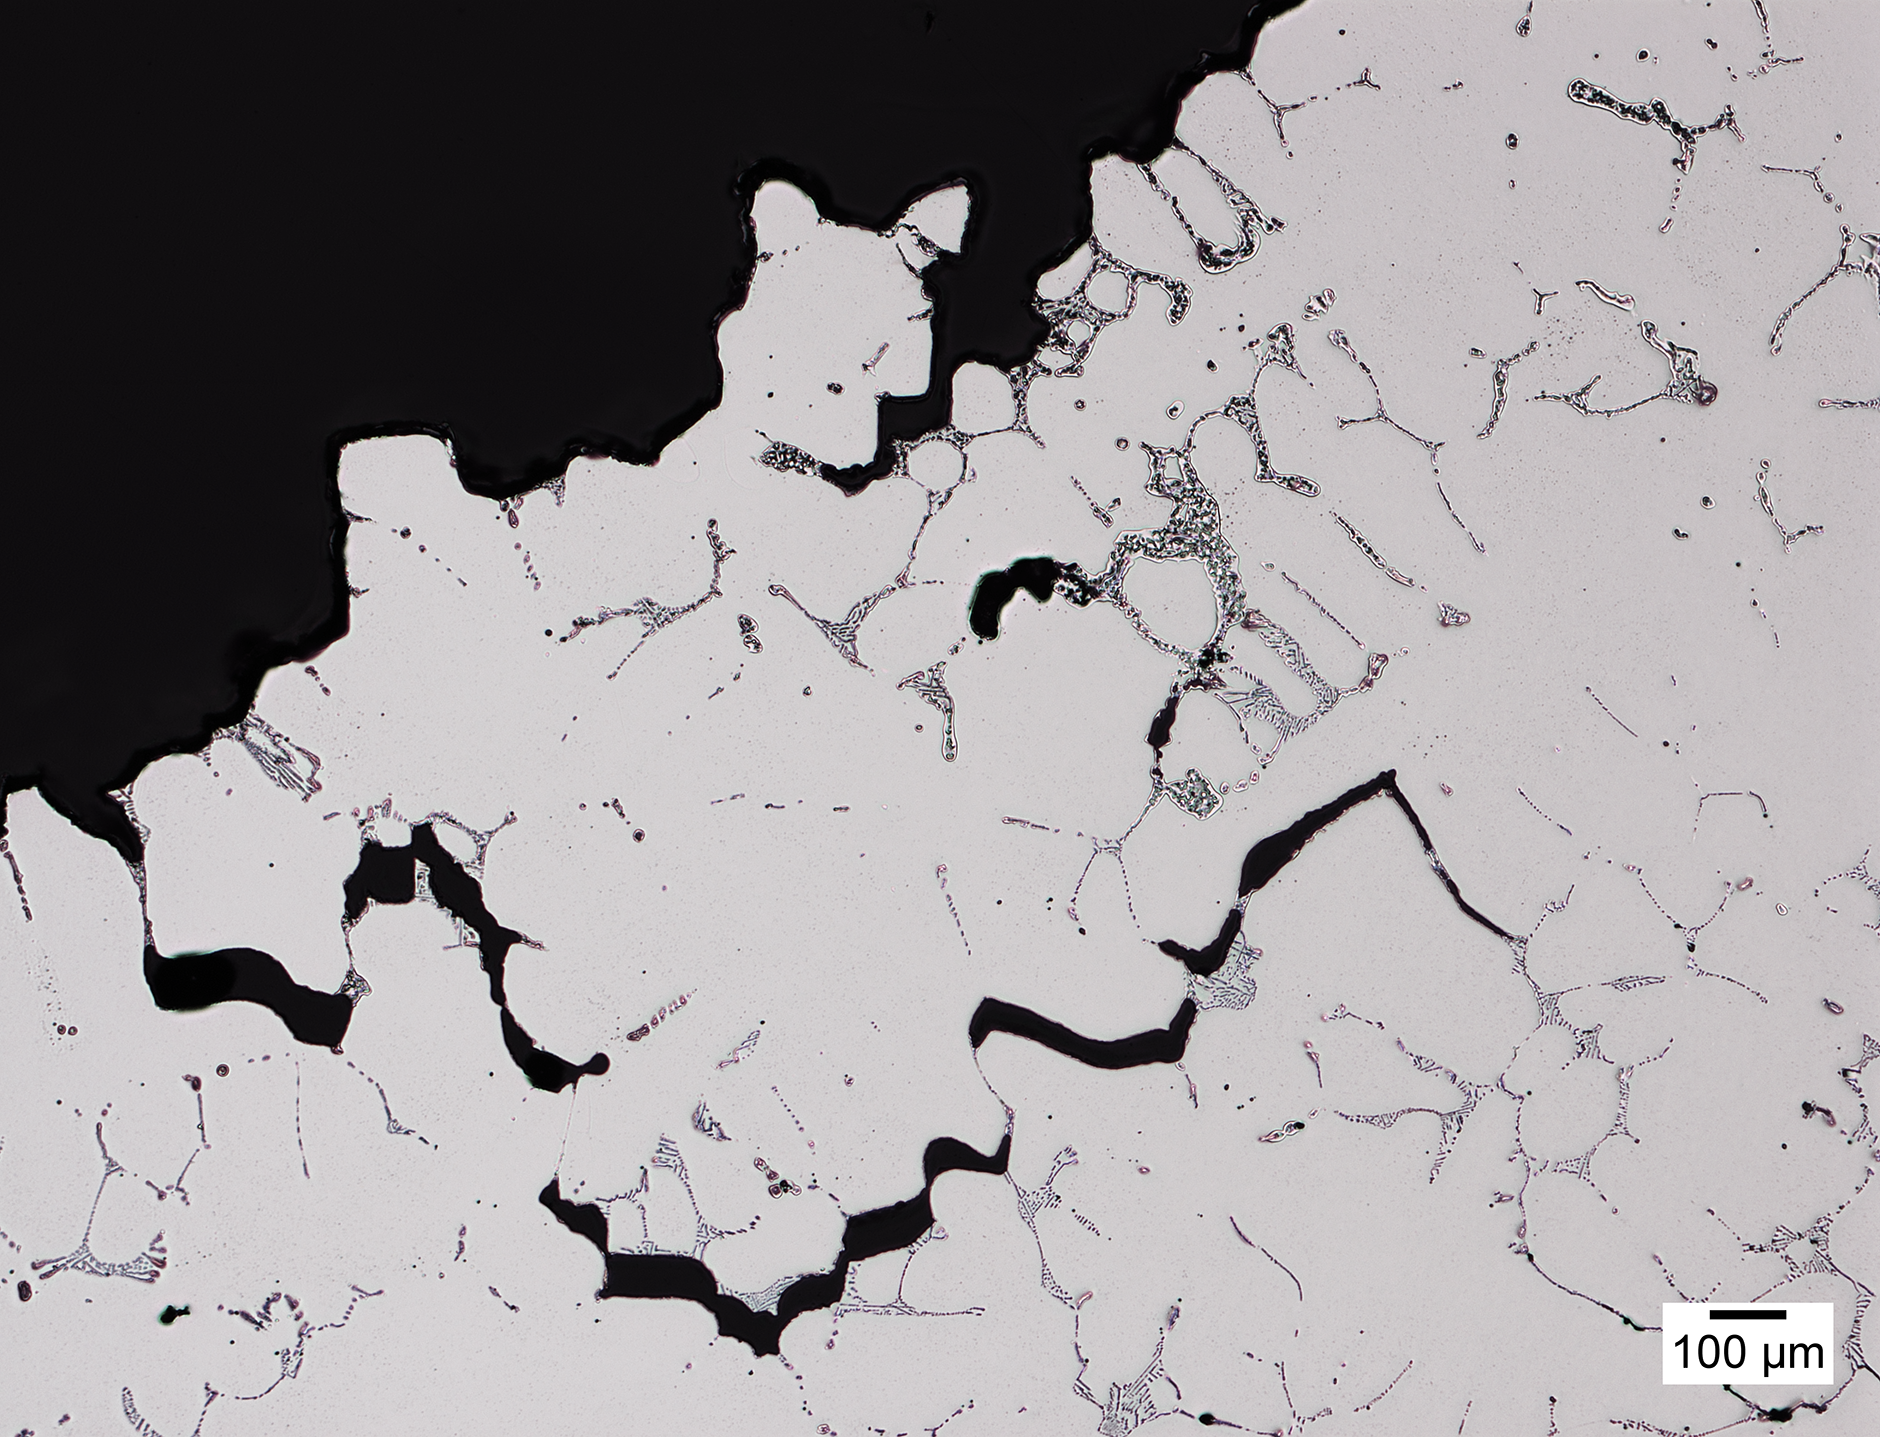
\includegraphics[width=4.7in]{figures/metallography/c1-oh-2375-50x.png}} \\
    \subfloat[500X]{\label{subfig:c1-oh-2375-500X}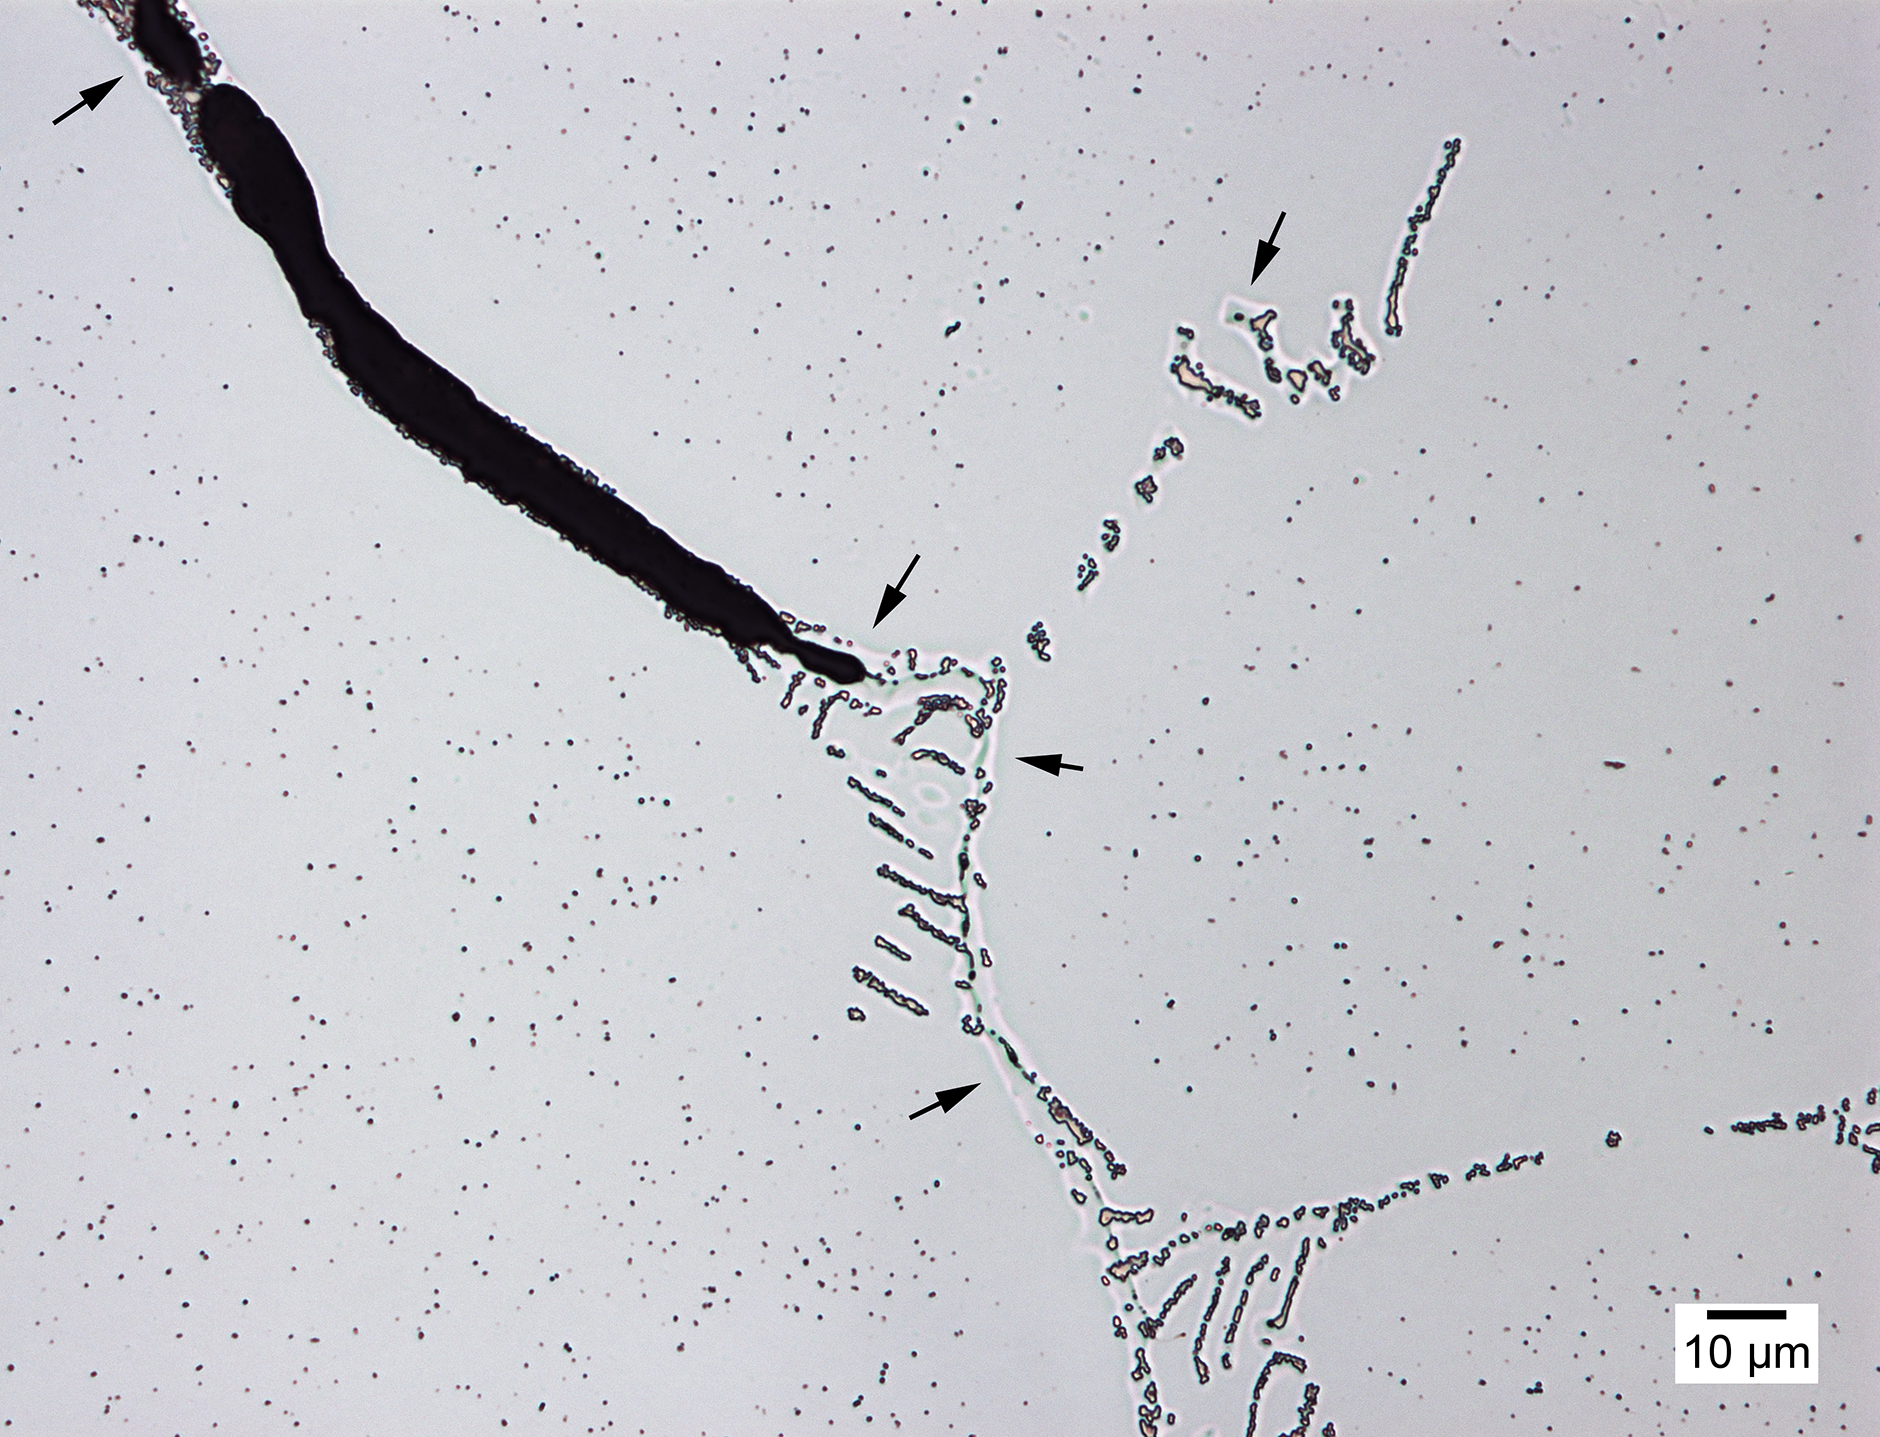
\includegraphics[width=4.7in]{figures/metallography/c1-oh-2375-crack-500x.png}}
    \caption{Optical micrographs showing the region adjacent to the fracture surface in the Cone~1 On-Heating 2375\textdegree{}F (C1 OH-2375) hot ductility sample. Evidence of liquation (where melting occurred during the simulated thermal cycle) is denoted by arrows. Etch: electrolytic 10\% oxalic acid.}
    \label{fig:c1-oh-2375}
\end{figure}

\begin{figure}
    \centering
    \subfloat[100X]{\label{subfig:c1-oh-2375-liquation-100x}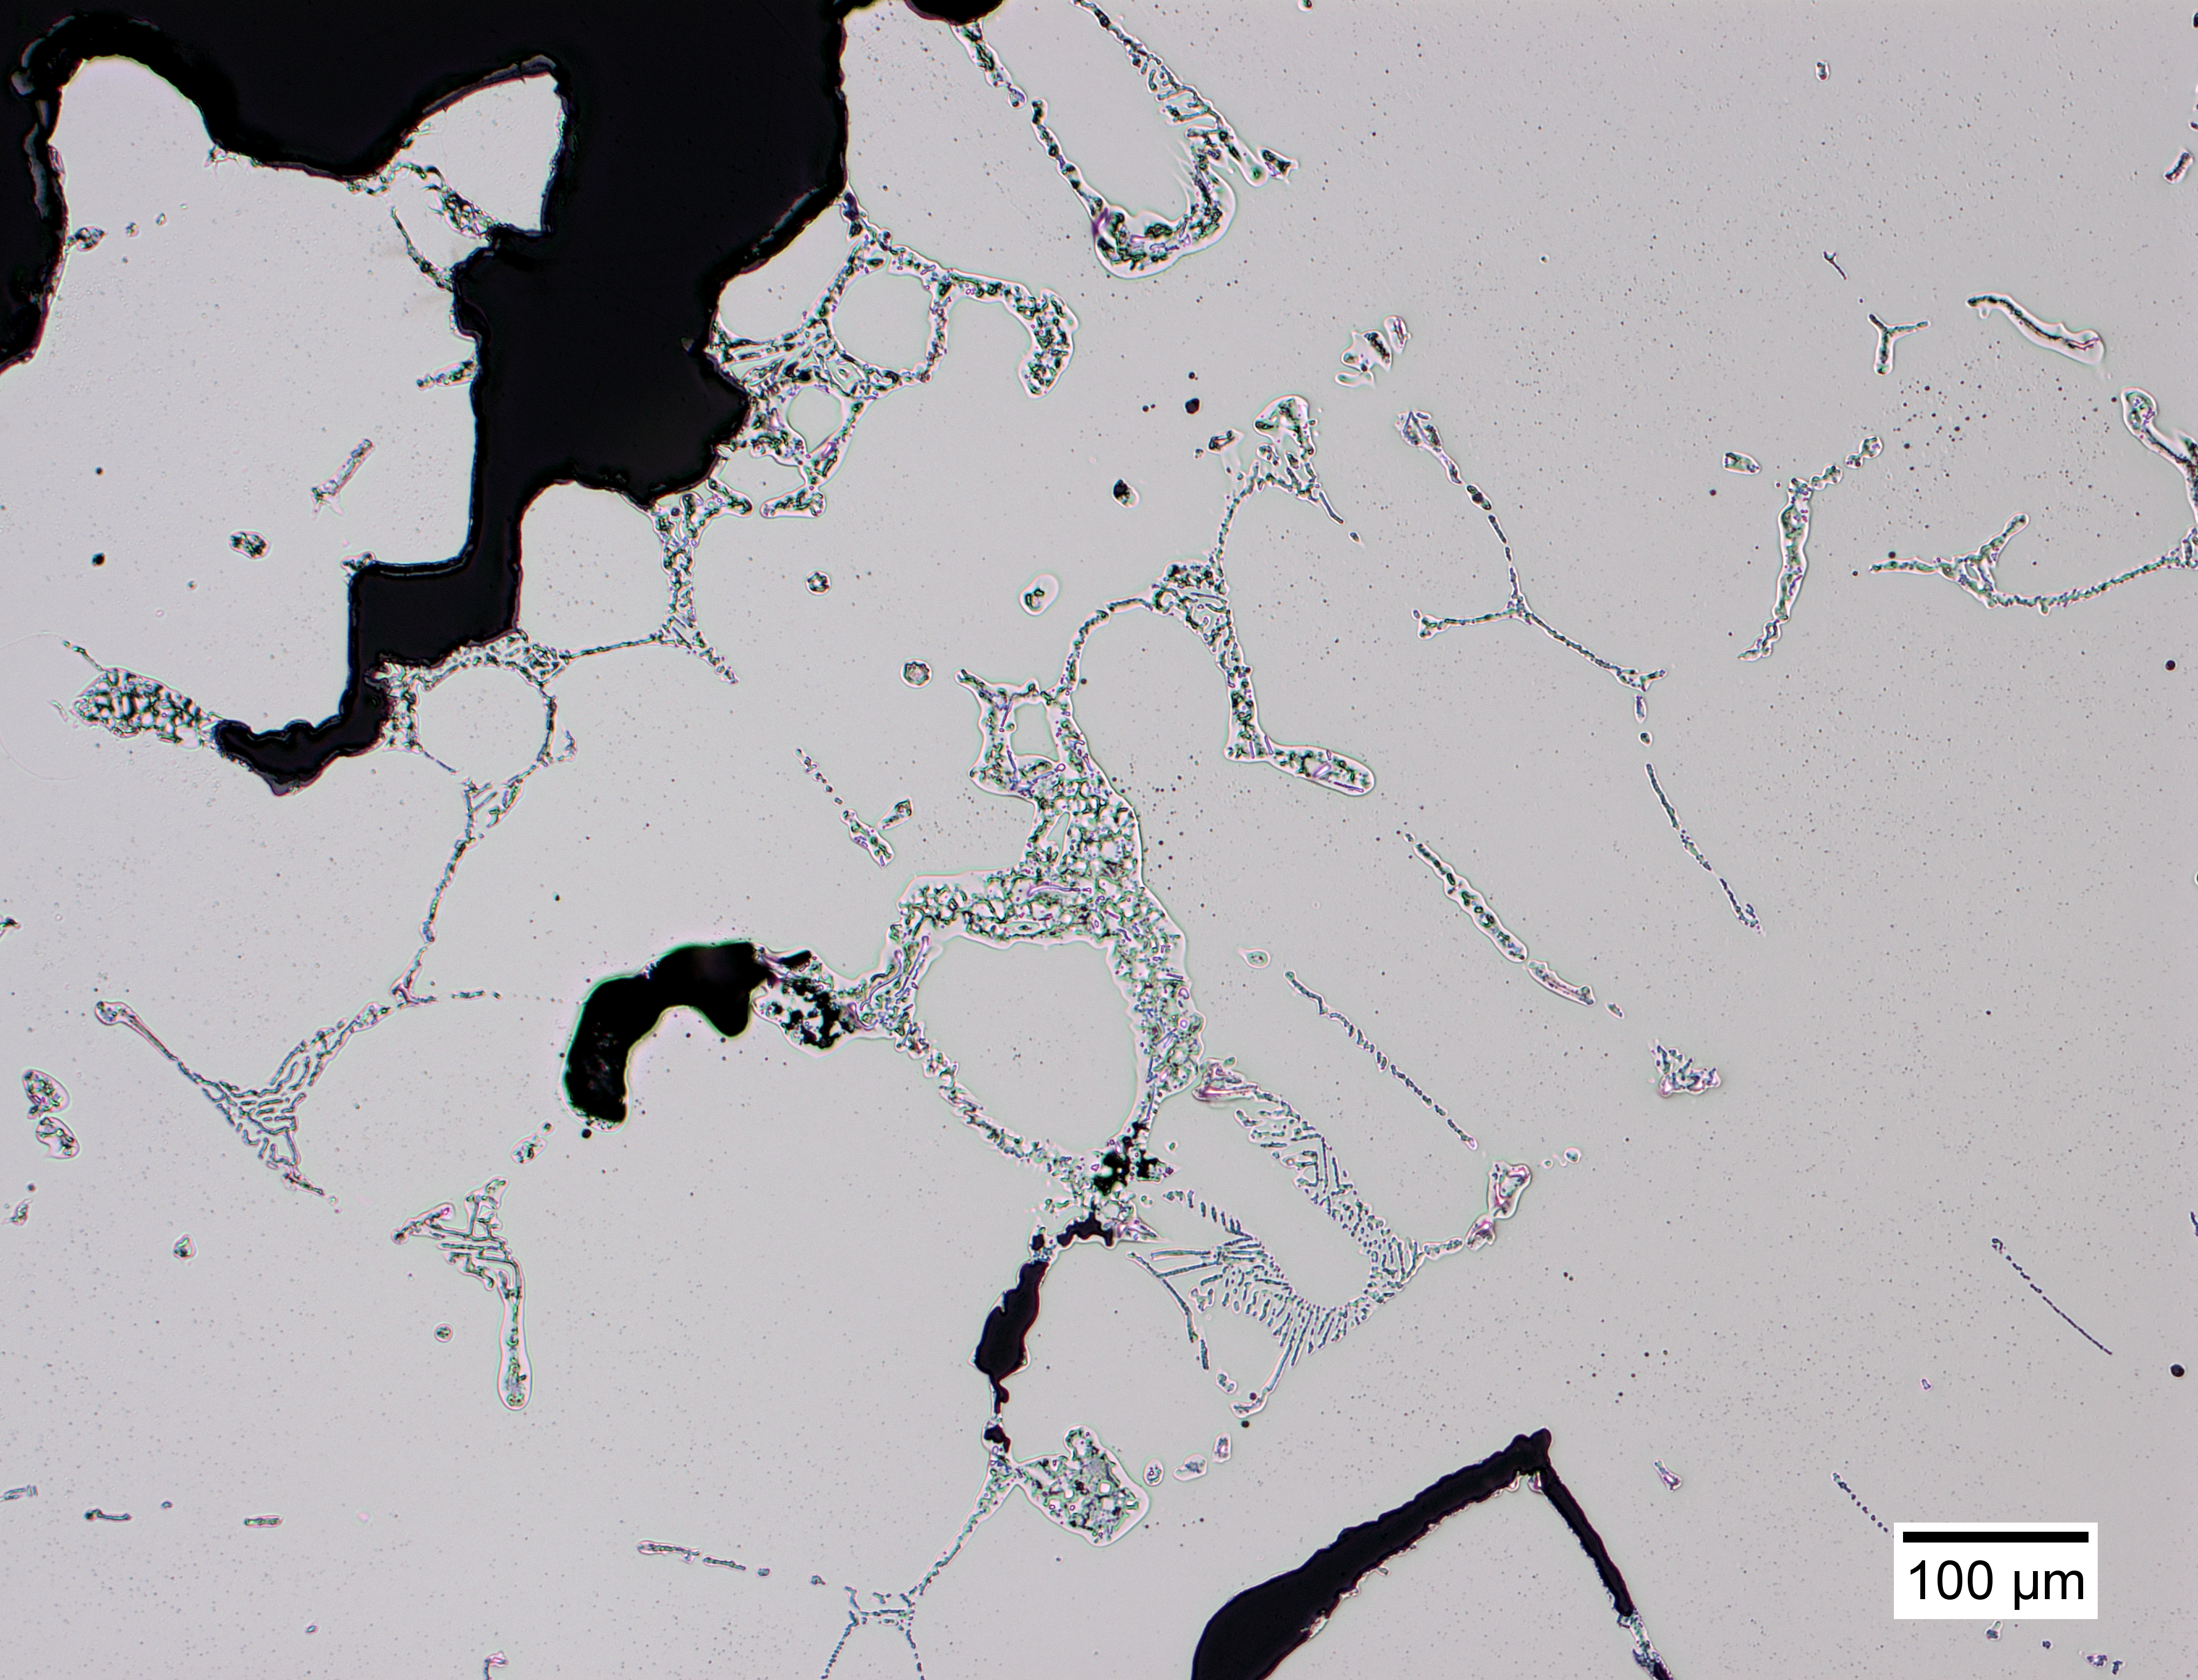
\includegraphics[width=4.7in]{figures/metallography/c1-oh-2375-fracture-liquation-100x.png}} \\
    \subfloat[500X]{\label{subfig:c1-oh-2375-liquation-500X}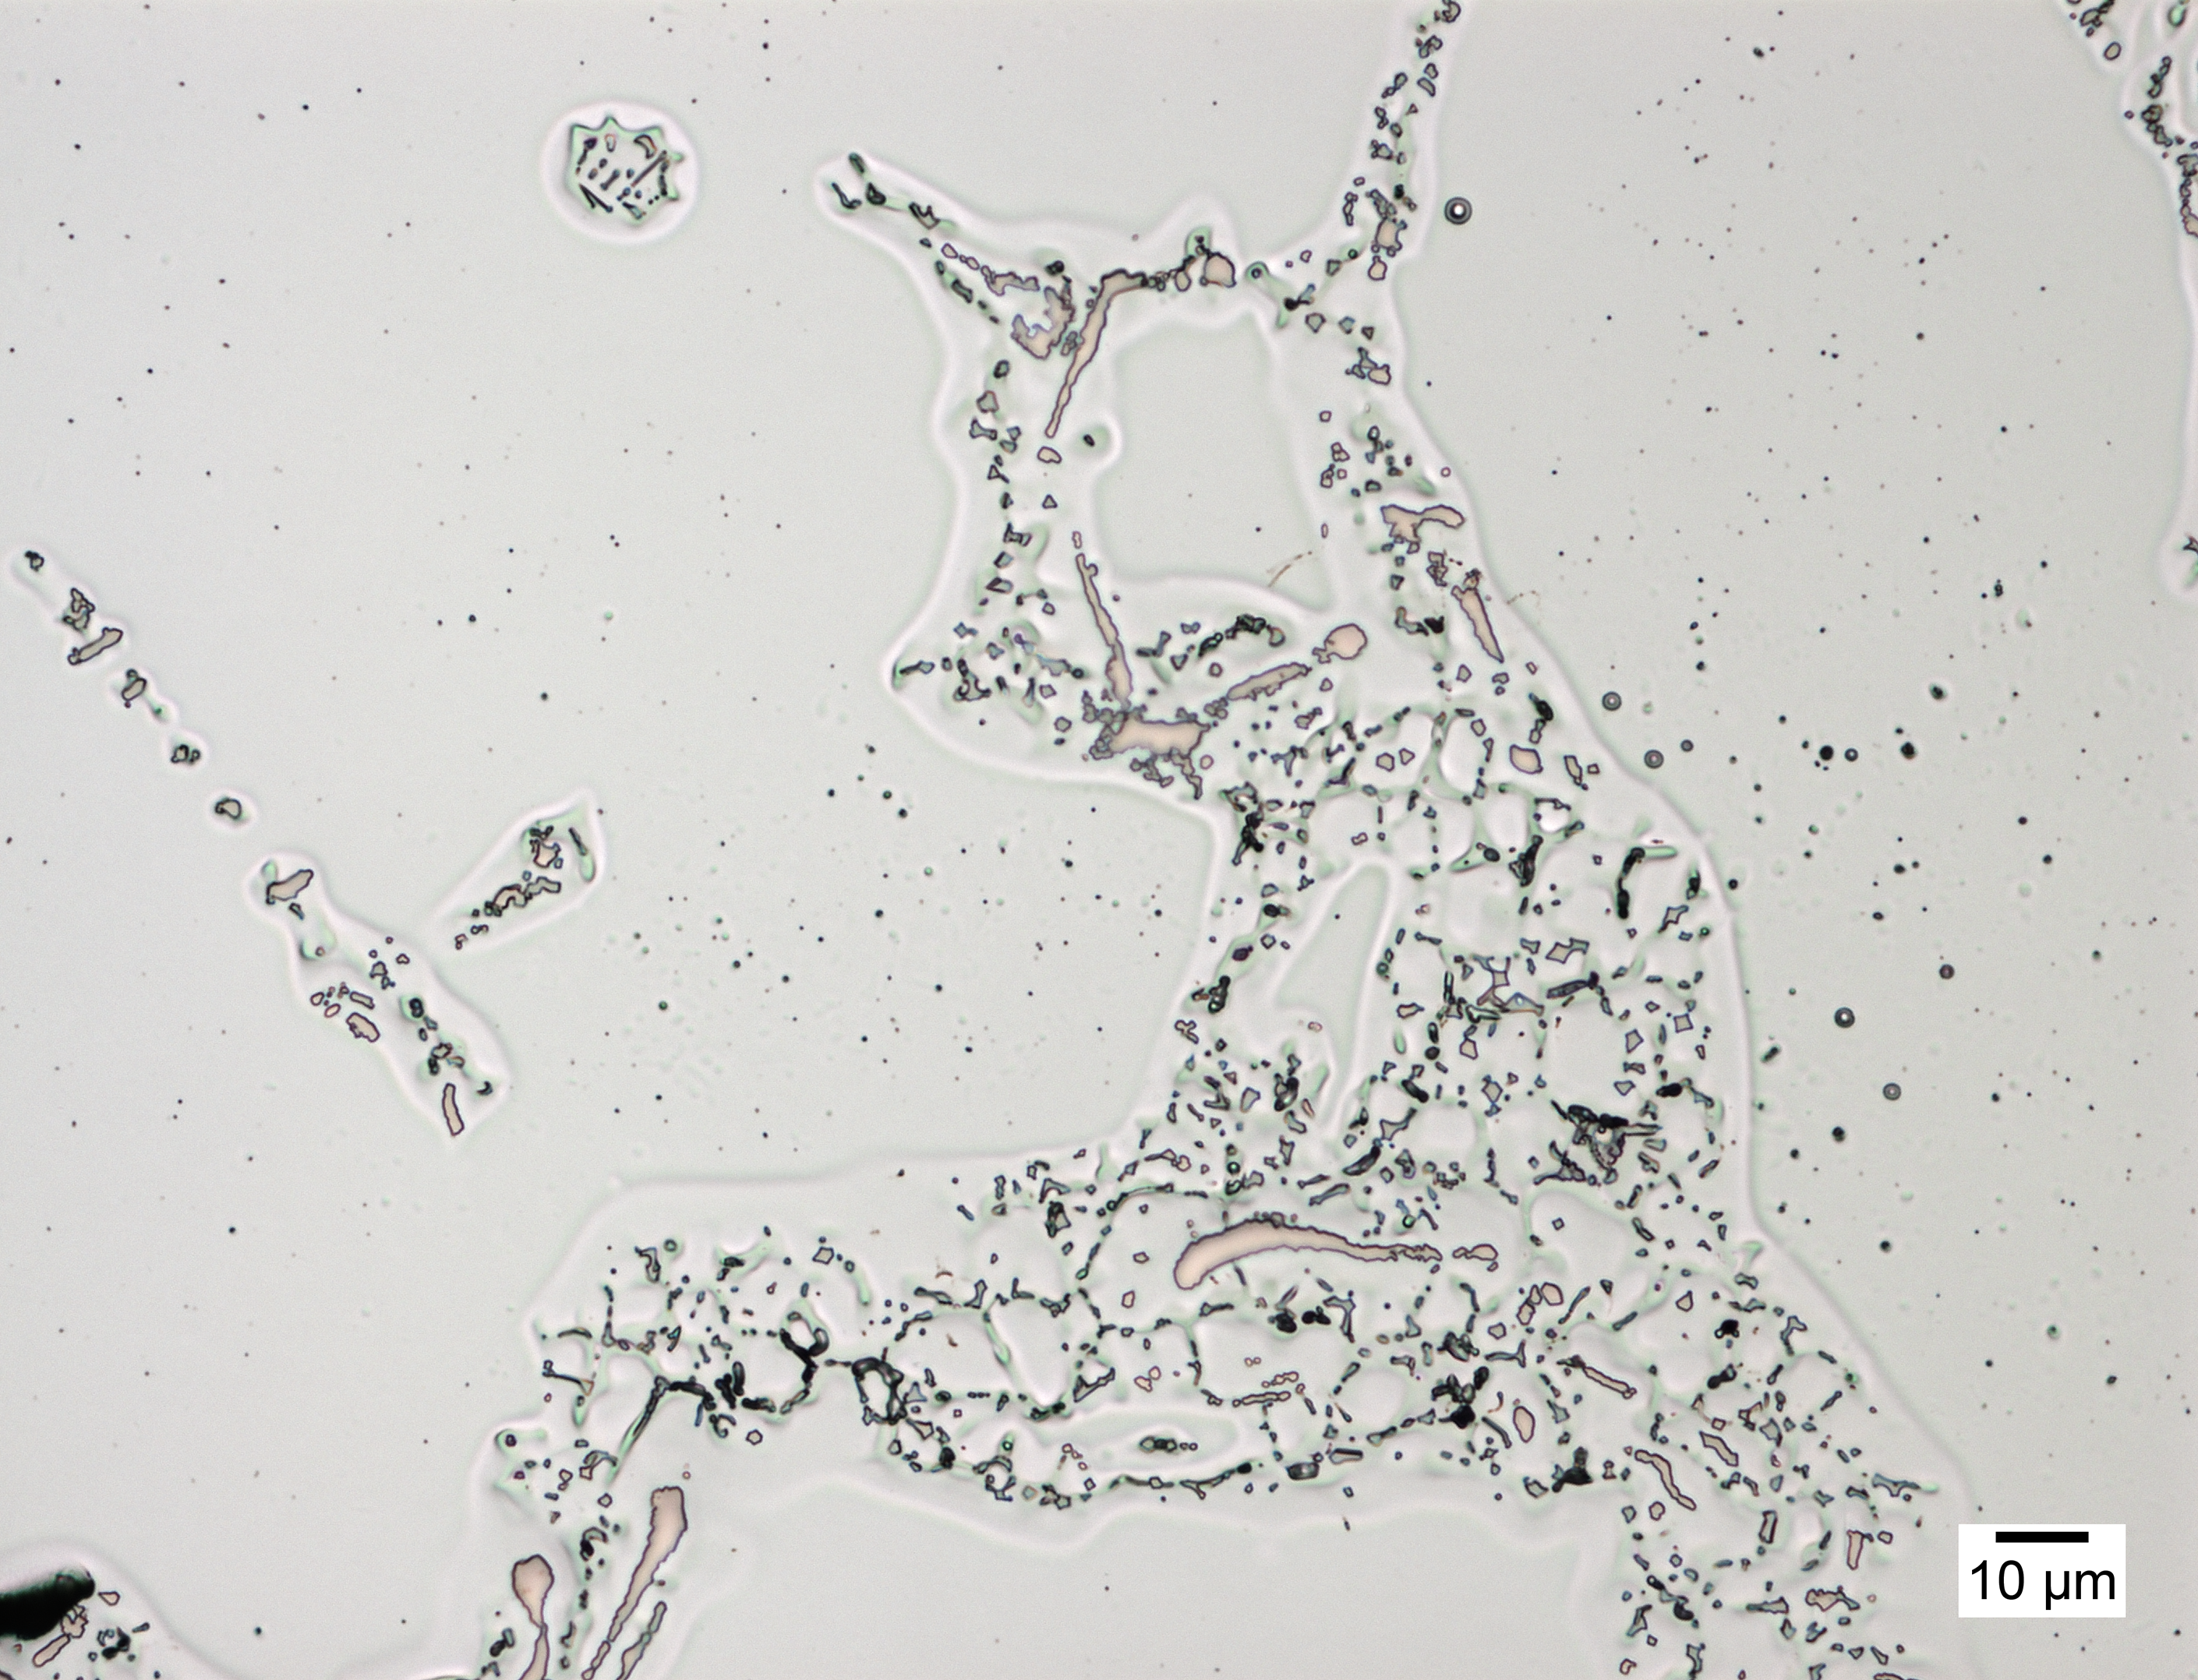
\includegraphics[width=4.7in]{figures/metallography/c1-oh-2375-fracture-liquation-500x.png}}
    \caption{Optical micrographs showing liquation around interdendritic phases adjacent to the fracture surface in the Cone~1 On-Heating 2375\textdegree{}F (C1 OH-2375) hot ductility sample. Etch: electrolytic 10\% oxalic acid.}
    \label{fig:c1-oh-2375-fracture-liquation}
\end{figure}

\begin{figure}
    \centering
    \subfloat[SEM micrograph of liquated region]{\label{subfig:c1-oh-2375-sem-2.5kx}\includegraphics[width=4.7in]{figures/metallography/c1-oh-2375-liquation-sem.png}} \\
    \subfloat[Spot \gls{eds} results for point ``A'']{\label{subfig:c1-oh-2375-liquation-eds}\includegraphics[width=\textwidth]{figures/metallography/c1-oh-2375-liquation-eds-table.png}}
    \caption{\Gls{sem} micrograph showing liquation around interdendritic phases adjacent to the fracture surface in the Cone~1 On-Heating 2375\textdegree{}F (C1 OH-2375) hot ductility sample with spot \gls{eds} results for indicated point ``A'' within the melted region. Etch: electrolytic 10\% oxalic acid.}
    \label{fig:c1-oh-2375-fracture-liquation-sem}
\end{figure}
\clearpage
%Need some EDS of phases in front of crack, e.g. NbC

\subsubsection{Cone~5 On-Heating}
Figure~\ref{fig:c5-oh-2375-olm-fracture} shows a region at the fracture surface of the Cone~5 On-Heating 2375\textdegree{}F (C5 OH-2375) hot ductility sample which corresponds to the \gls{ndt} of Cone~5. As with Cone~1, cracking is evident along the interdendritic boundaries and a majority of the intradendritic precipitates have dissolved due to the high temperature exposure. The crack tip is shown in Figure~\ref{fig:c5-oh-2375-crack-100x} and two separate regions at the tip of the crack shown in Figure~\ref{fig:c5-oh-2375-crack-100x} are shown at higher magnification in Figure~\ref{fig:c5-oh-2375-crack-tip-500x}. It is apparent that liquated regions (where liquid was formed during the simulated thermal cycle) exist along a portion of the crack faces and around some of the interdendritic phases ahead of the crack (see arrows in Figure~\ref{subfig:c5-oh-2375-wide-crack-500x}). However, significant evidence of liquid is not apparent at the extreme tip portion where the crack is quite narrow (Figure~\ref{subfig:c5-oh-2375-narrow-crack-500x}), indicating that minimal to no liquid was formed at this location during the simulated thermal cycle. Similarly to Cone~1, liquated regions are visible at other locations adjacent to the fracture surface away from apparent cracks, as shown in Figure~\ref{fig:c5-oh-2375-liquation-fracture-surface}. Again, the liquated regions are not present continuously along the fracture profile, indicating a lesser extent of liquid formation (as compared to the on-cooling tests which will be discussed later). Overall, both Cone~1 and Cone~5 show a similar hot ductility response in the on-heating tests.

%[C5 OH-2375 SEM to be added]

%Figures for C5 OH-2375
\begin{figure}
    \centering
    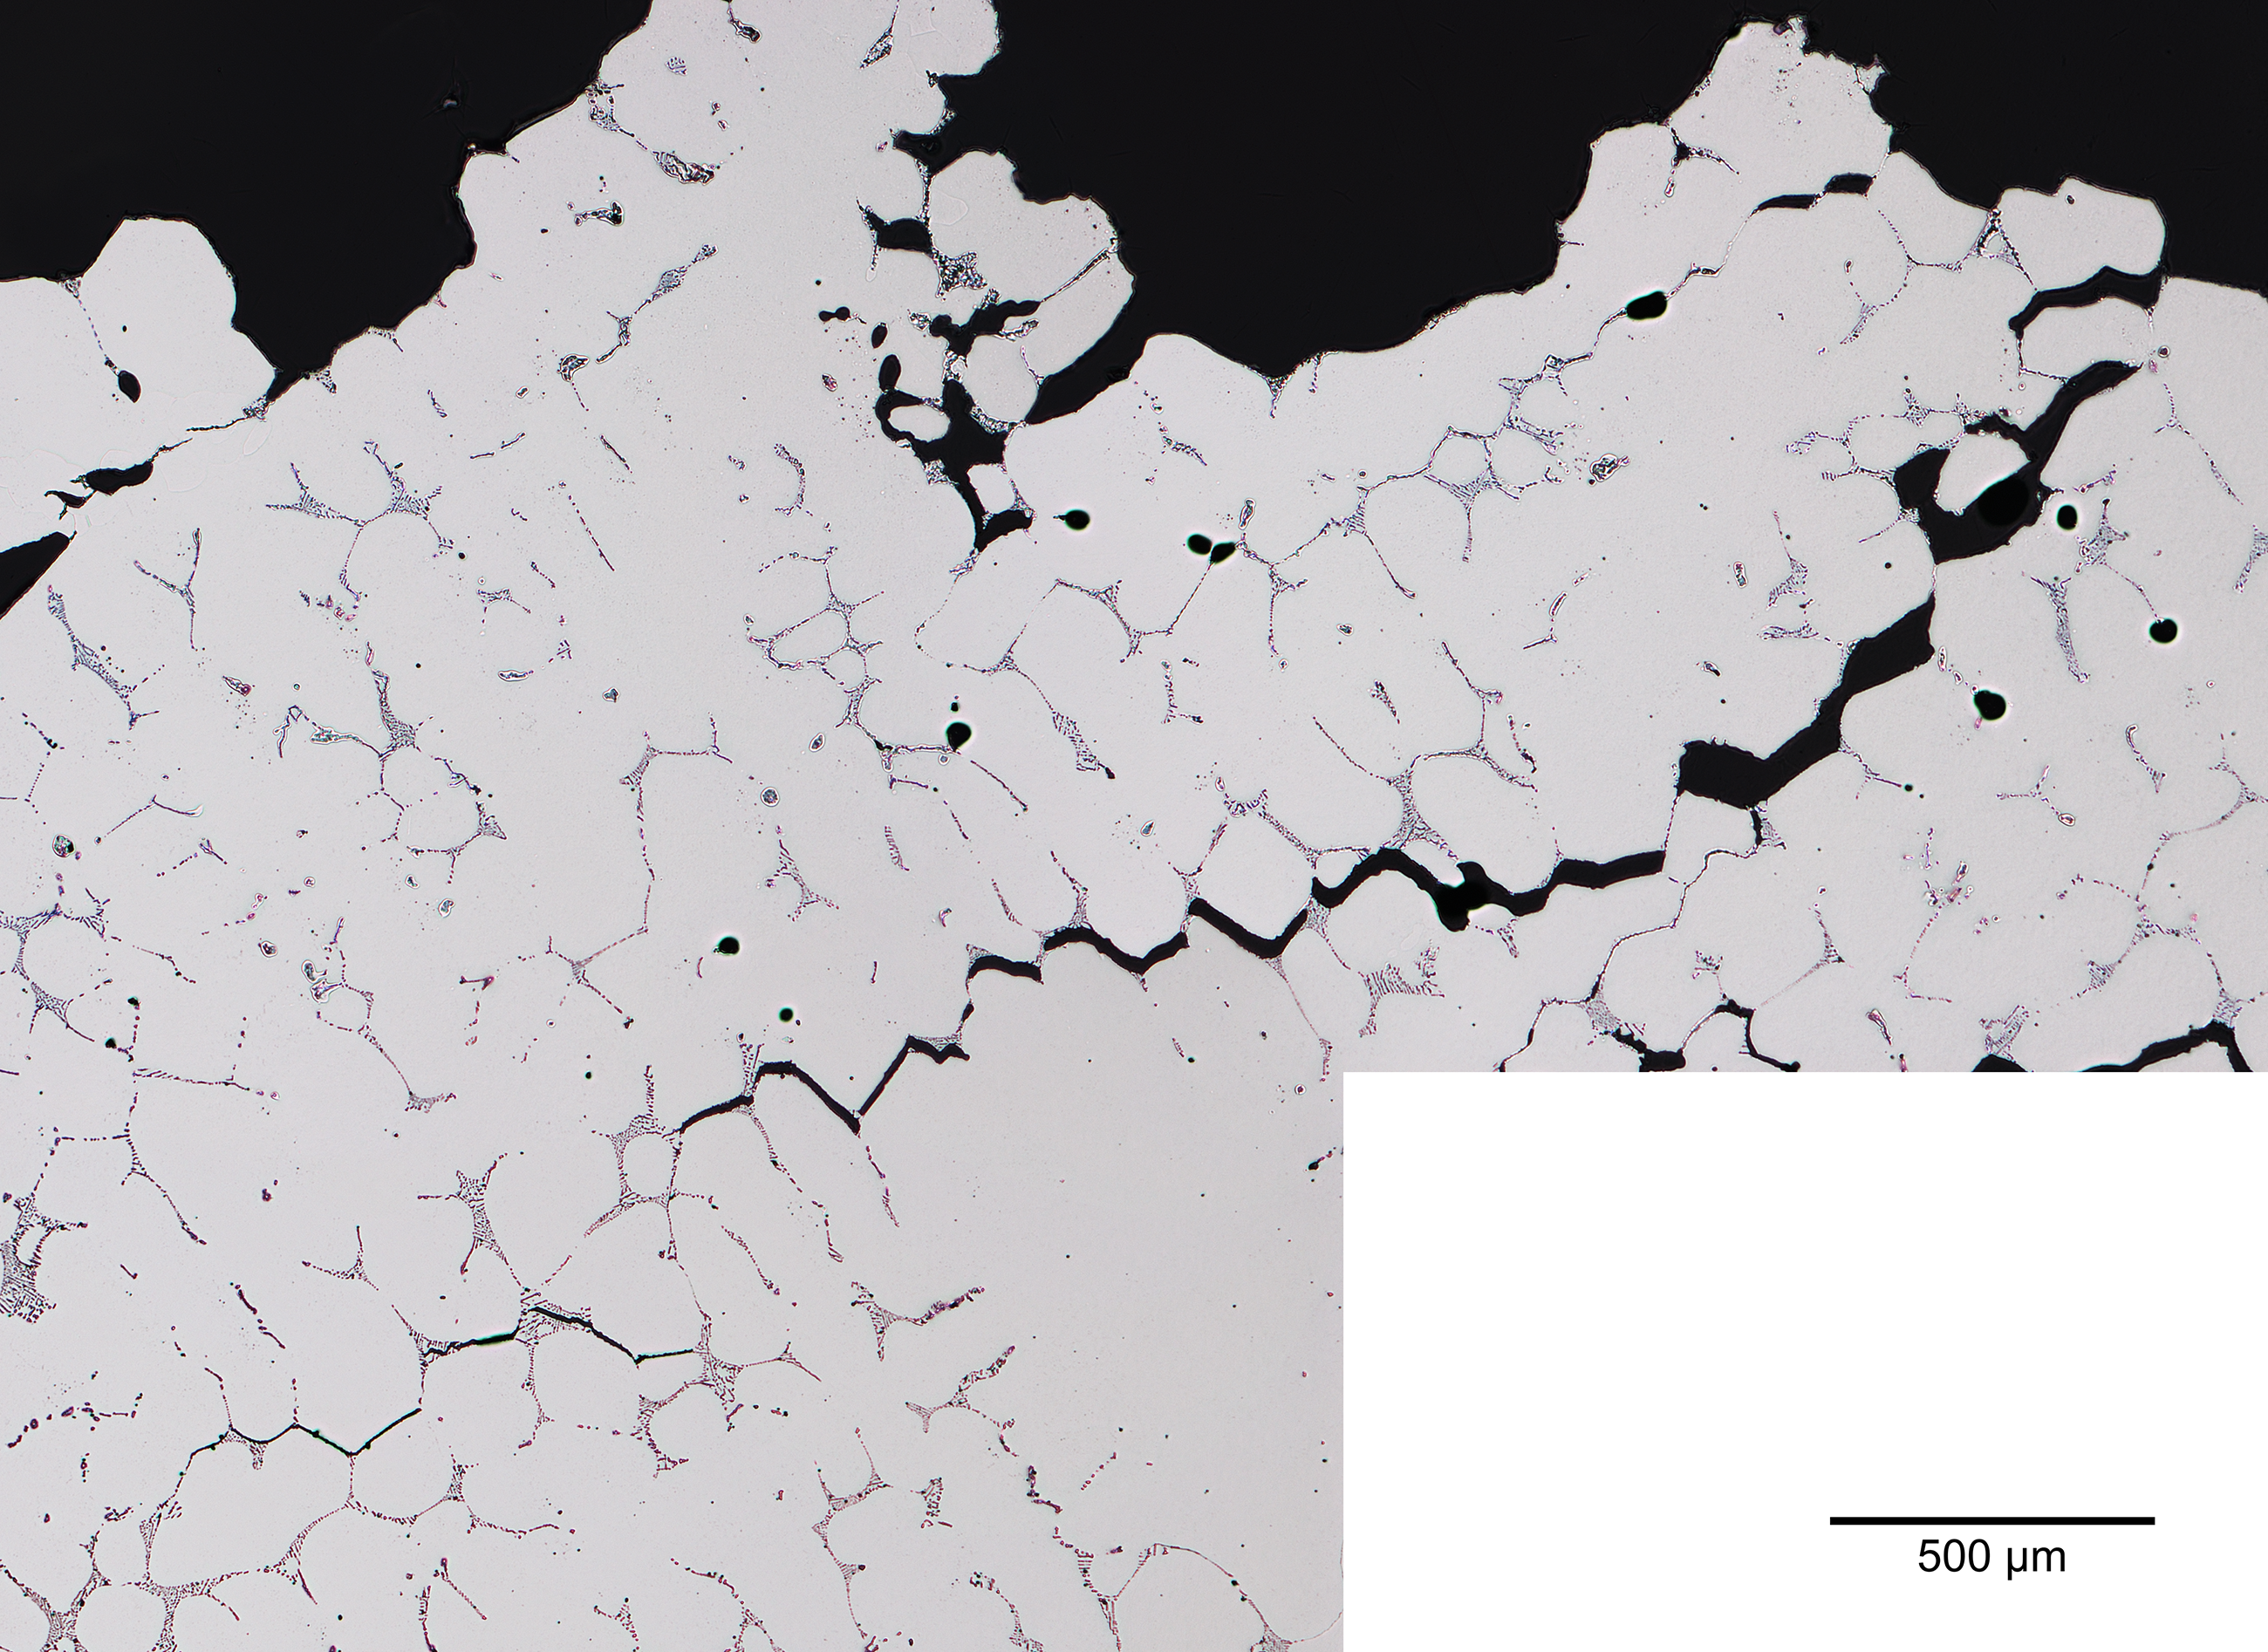
\includegraphics[width=\textwidth]{figures/metallography/c5-oh-2375-olm-fracture-50x.png}
    \caption{Optical micrograph showing cracking and liquation in a region adjacent to the fracture surface in the Cone~5 On-Heating 2375\textdegree{}F (C5 OH-2375) hot ductility sample. The crack tip region is shown in Figure~\ref{fig:c5-oh-2375-crack-100x}. Etch: electrolytic 10\% oxalic acid.}
    \label{fig:c5-oh-2375-olm-fracture}
\end{figure}

\begin{figure}
    \centering
    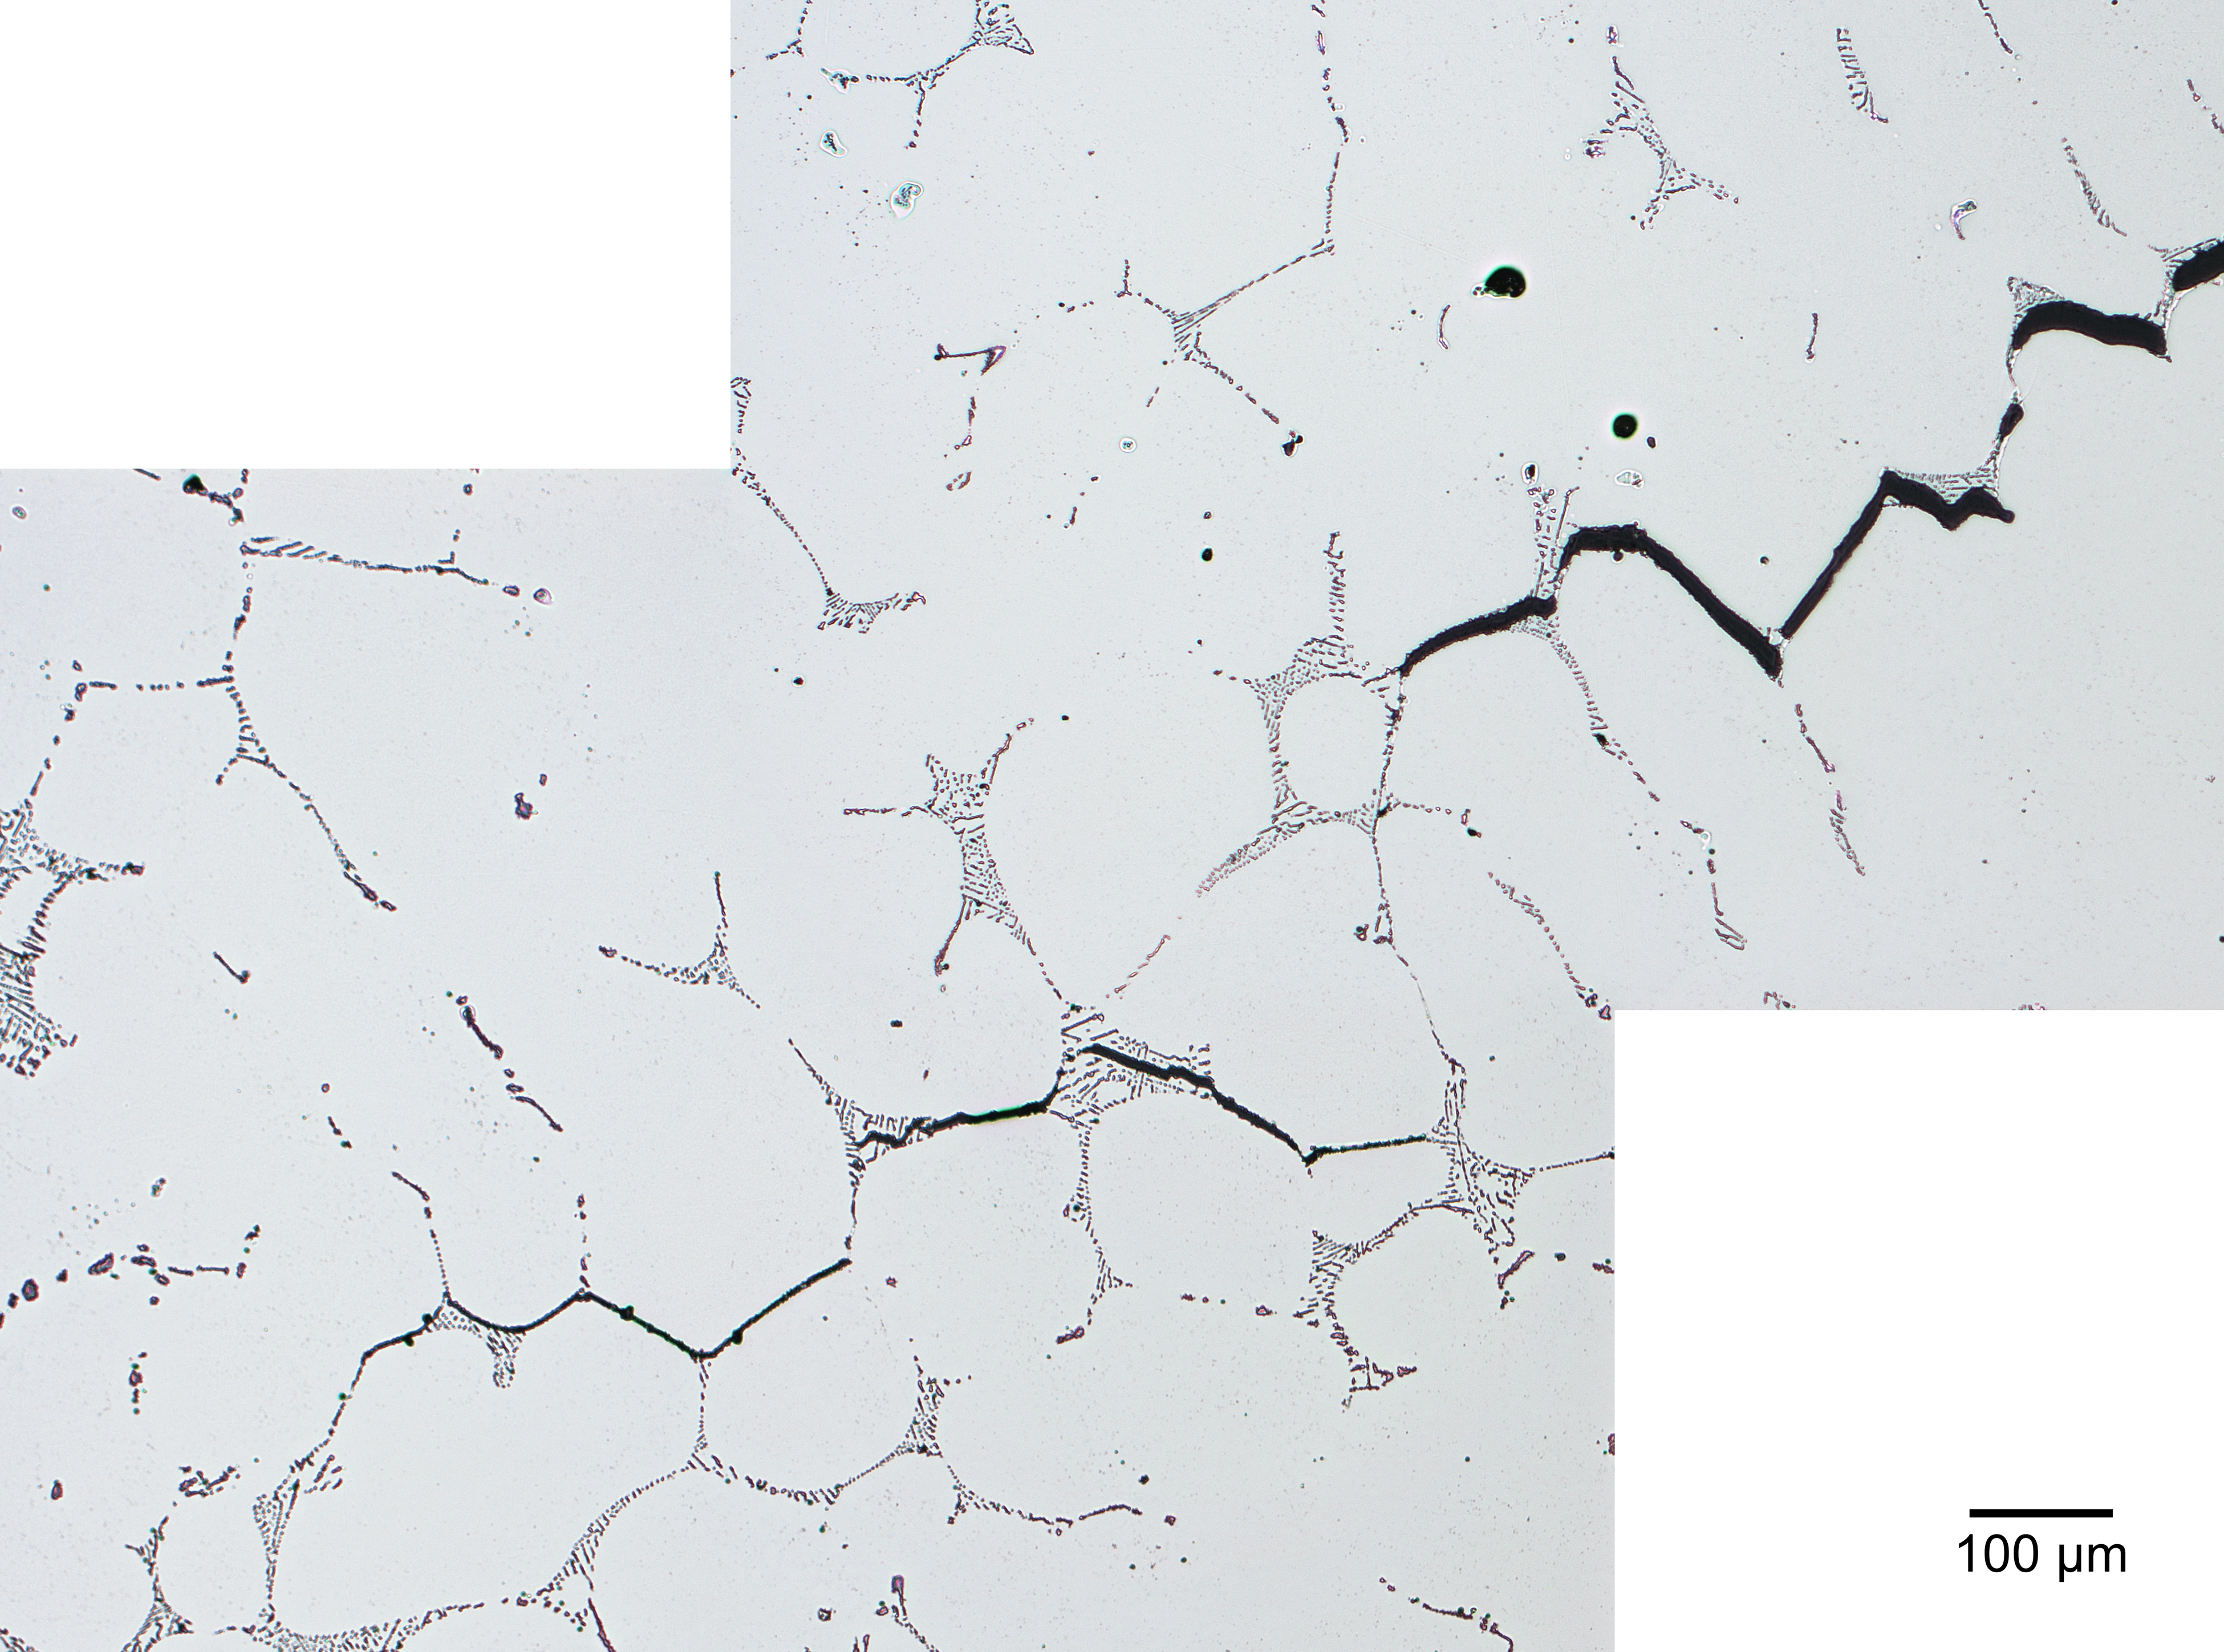
\includegraphics[width=\textwidth]{figures/metallography/c5-oh-2375-crack-100x.png}
    \caption{Optical micrograph of the tip of the crack visible in Figure~\ref{fig:c5-oh-2375-olm-fracture}. The crack tip region is shown at higher magnification in Figure~\ref{fig:c5-oh-2375-crack-tip-500x}. Etch: electrolytic 10\% oxalic acid.}
    \label{fig:c5-oh-2375-crack-100x}
\end{figure}

\begin{figure}
    \centering
    \subfloat[Wider region near crack tip]{\label{subfig:c5-oh-2375-wide-crack-500x}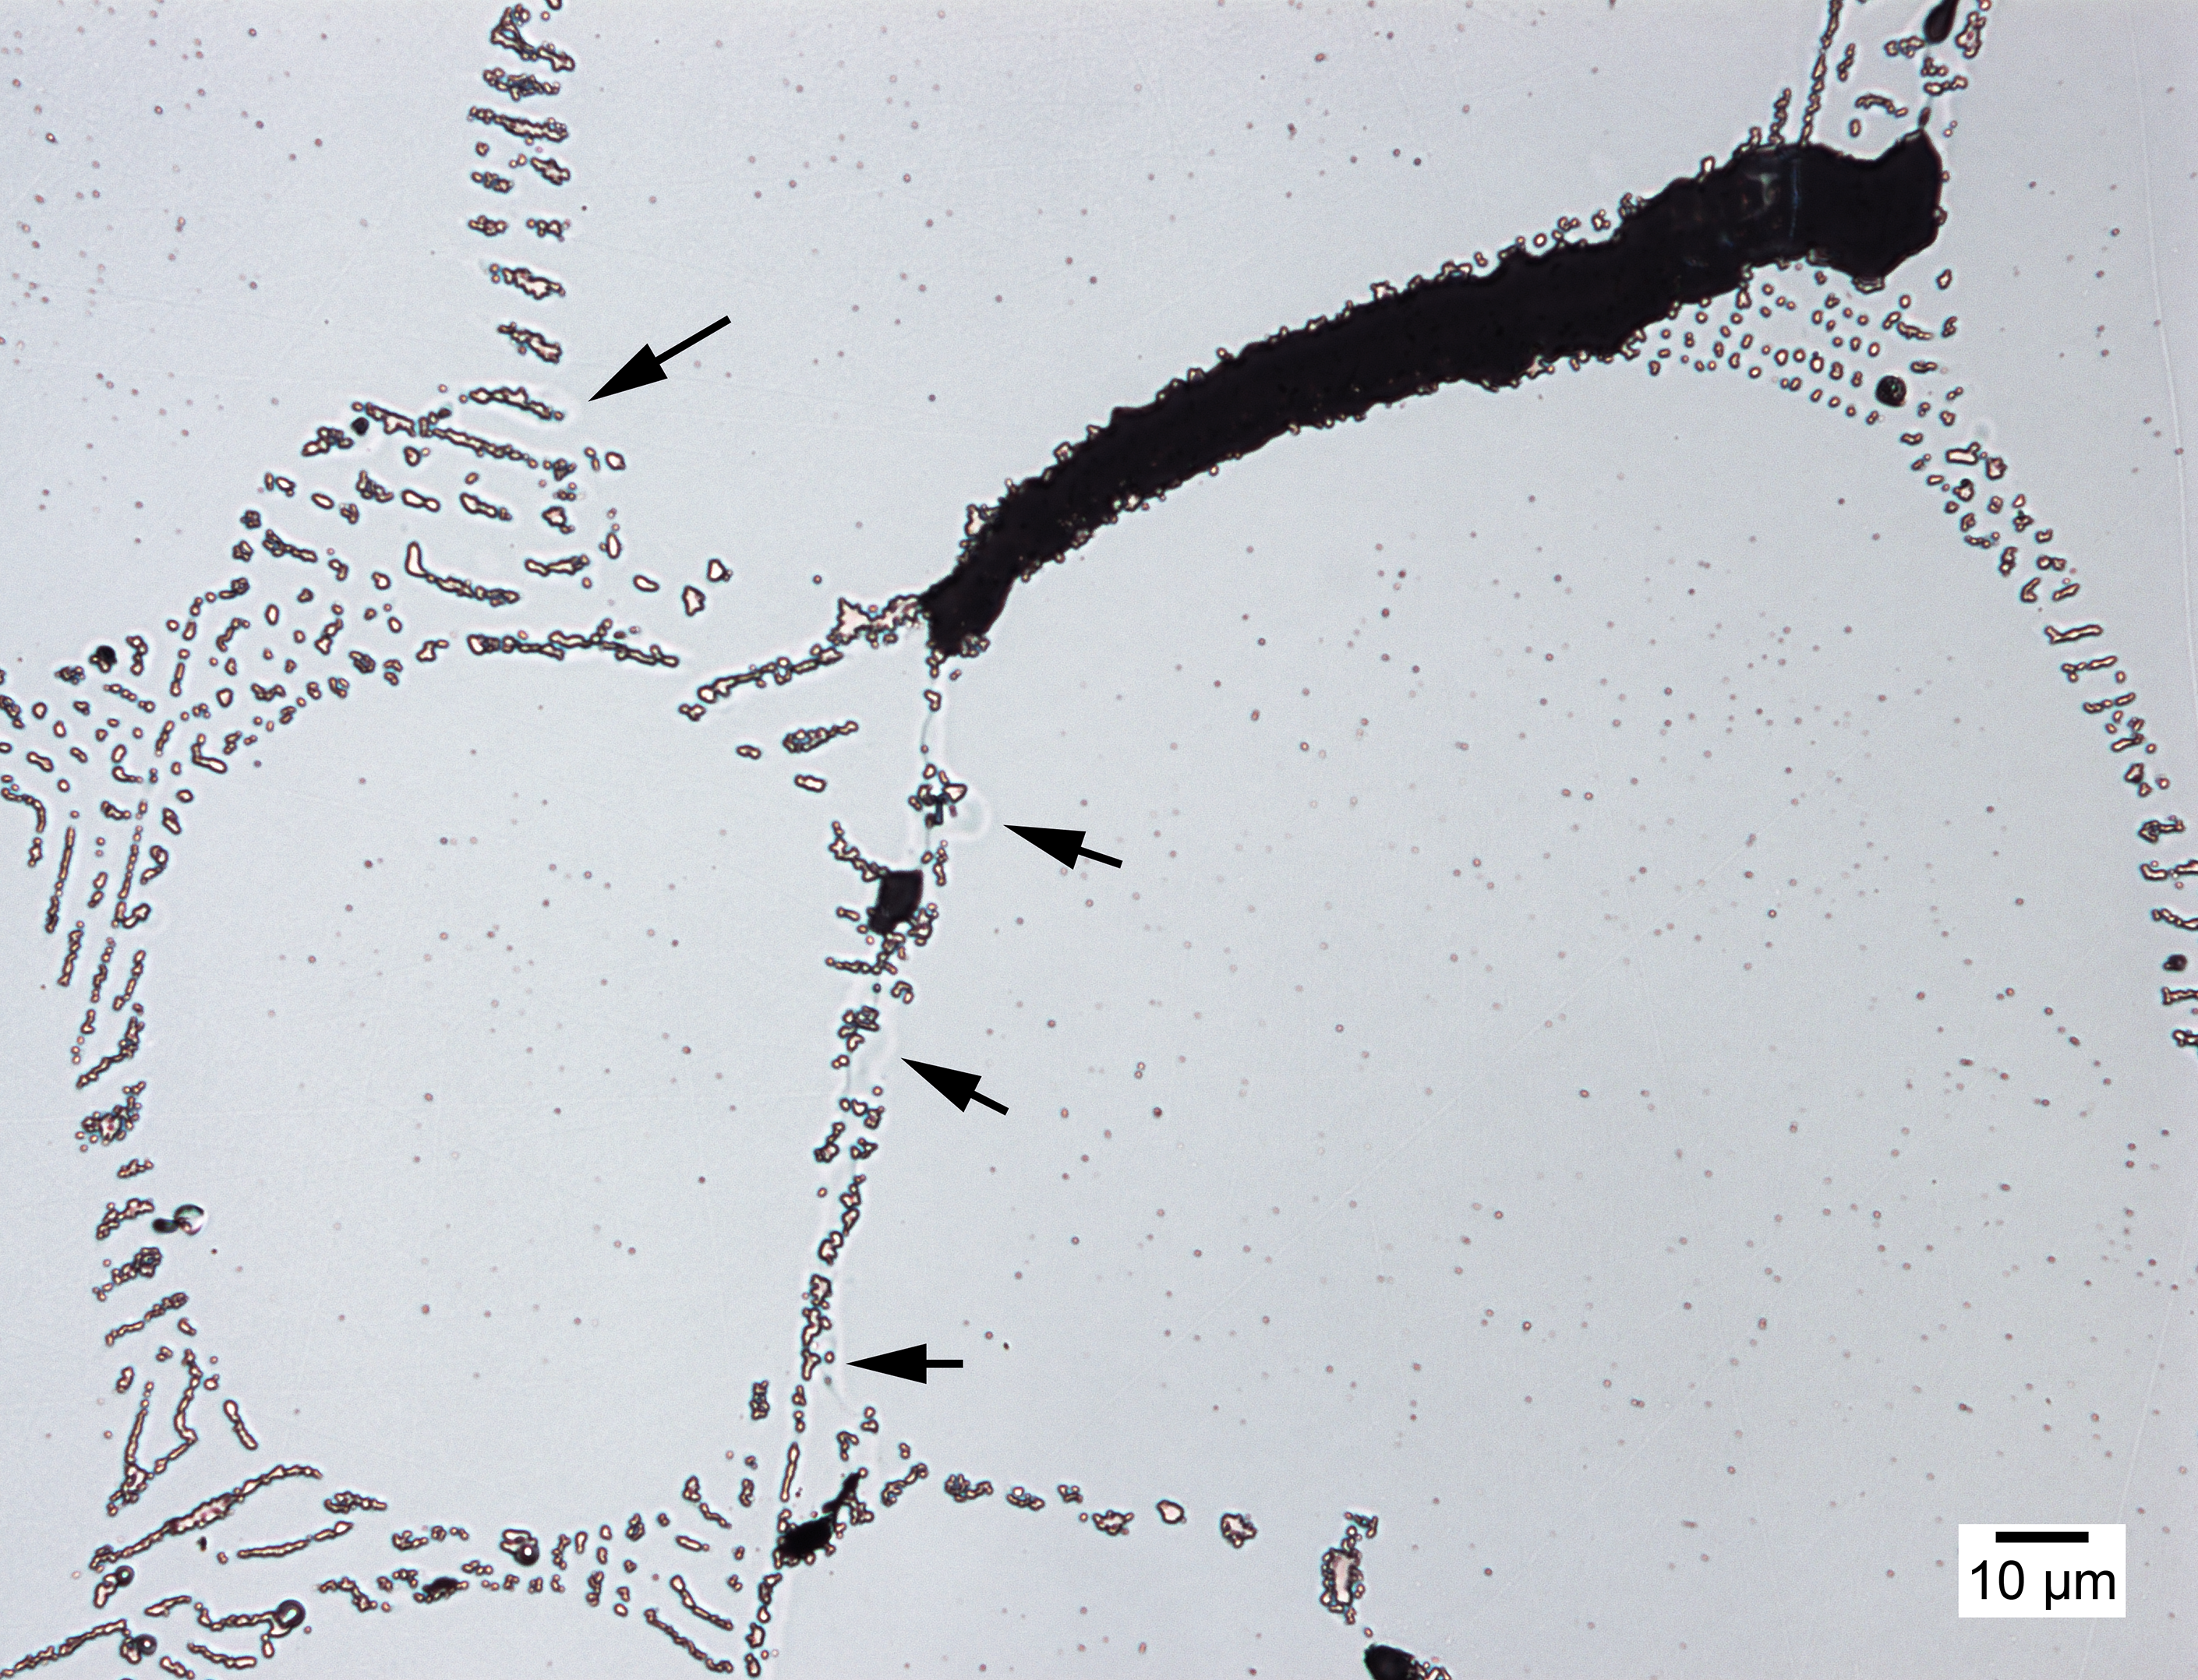
\includegraphics[width=4.7in]{figures/metallography/c5-oh-2375-wide-crack-500x.png}} \\
    \subfloat[Narrower region at crack tip]{\label{subfig:c5-oh-2375-narrow-crack-500x}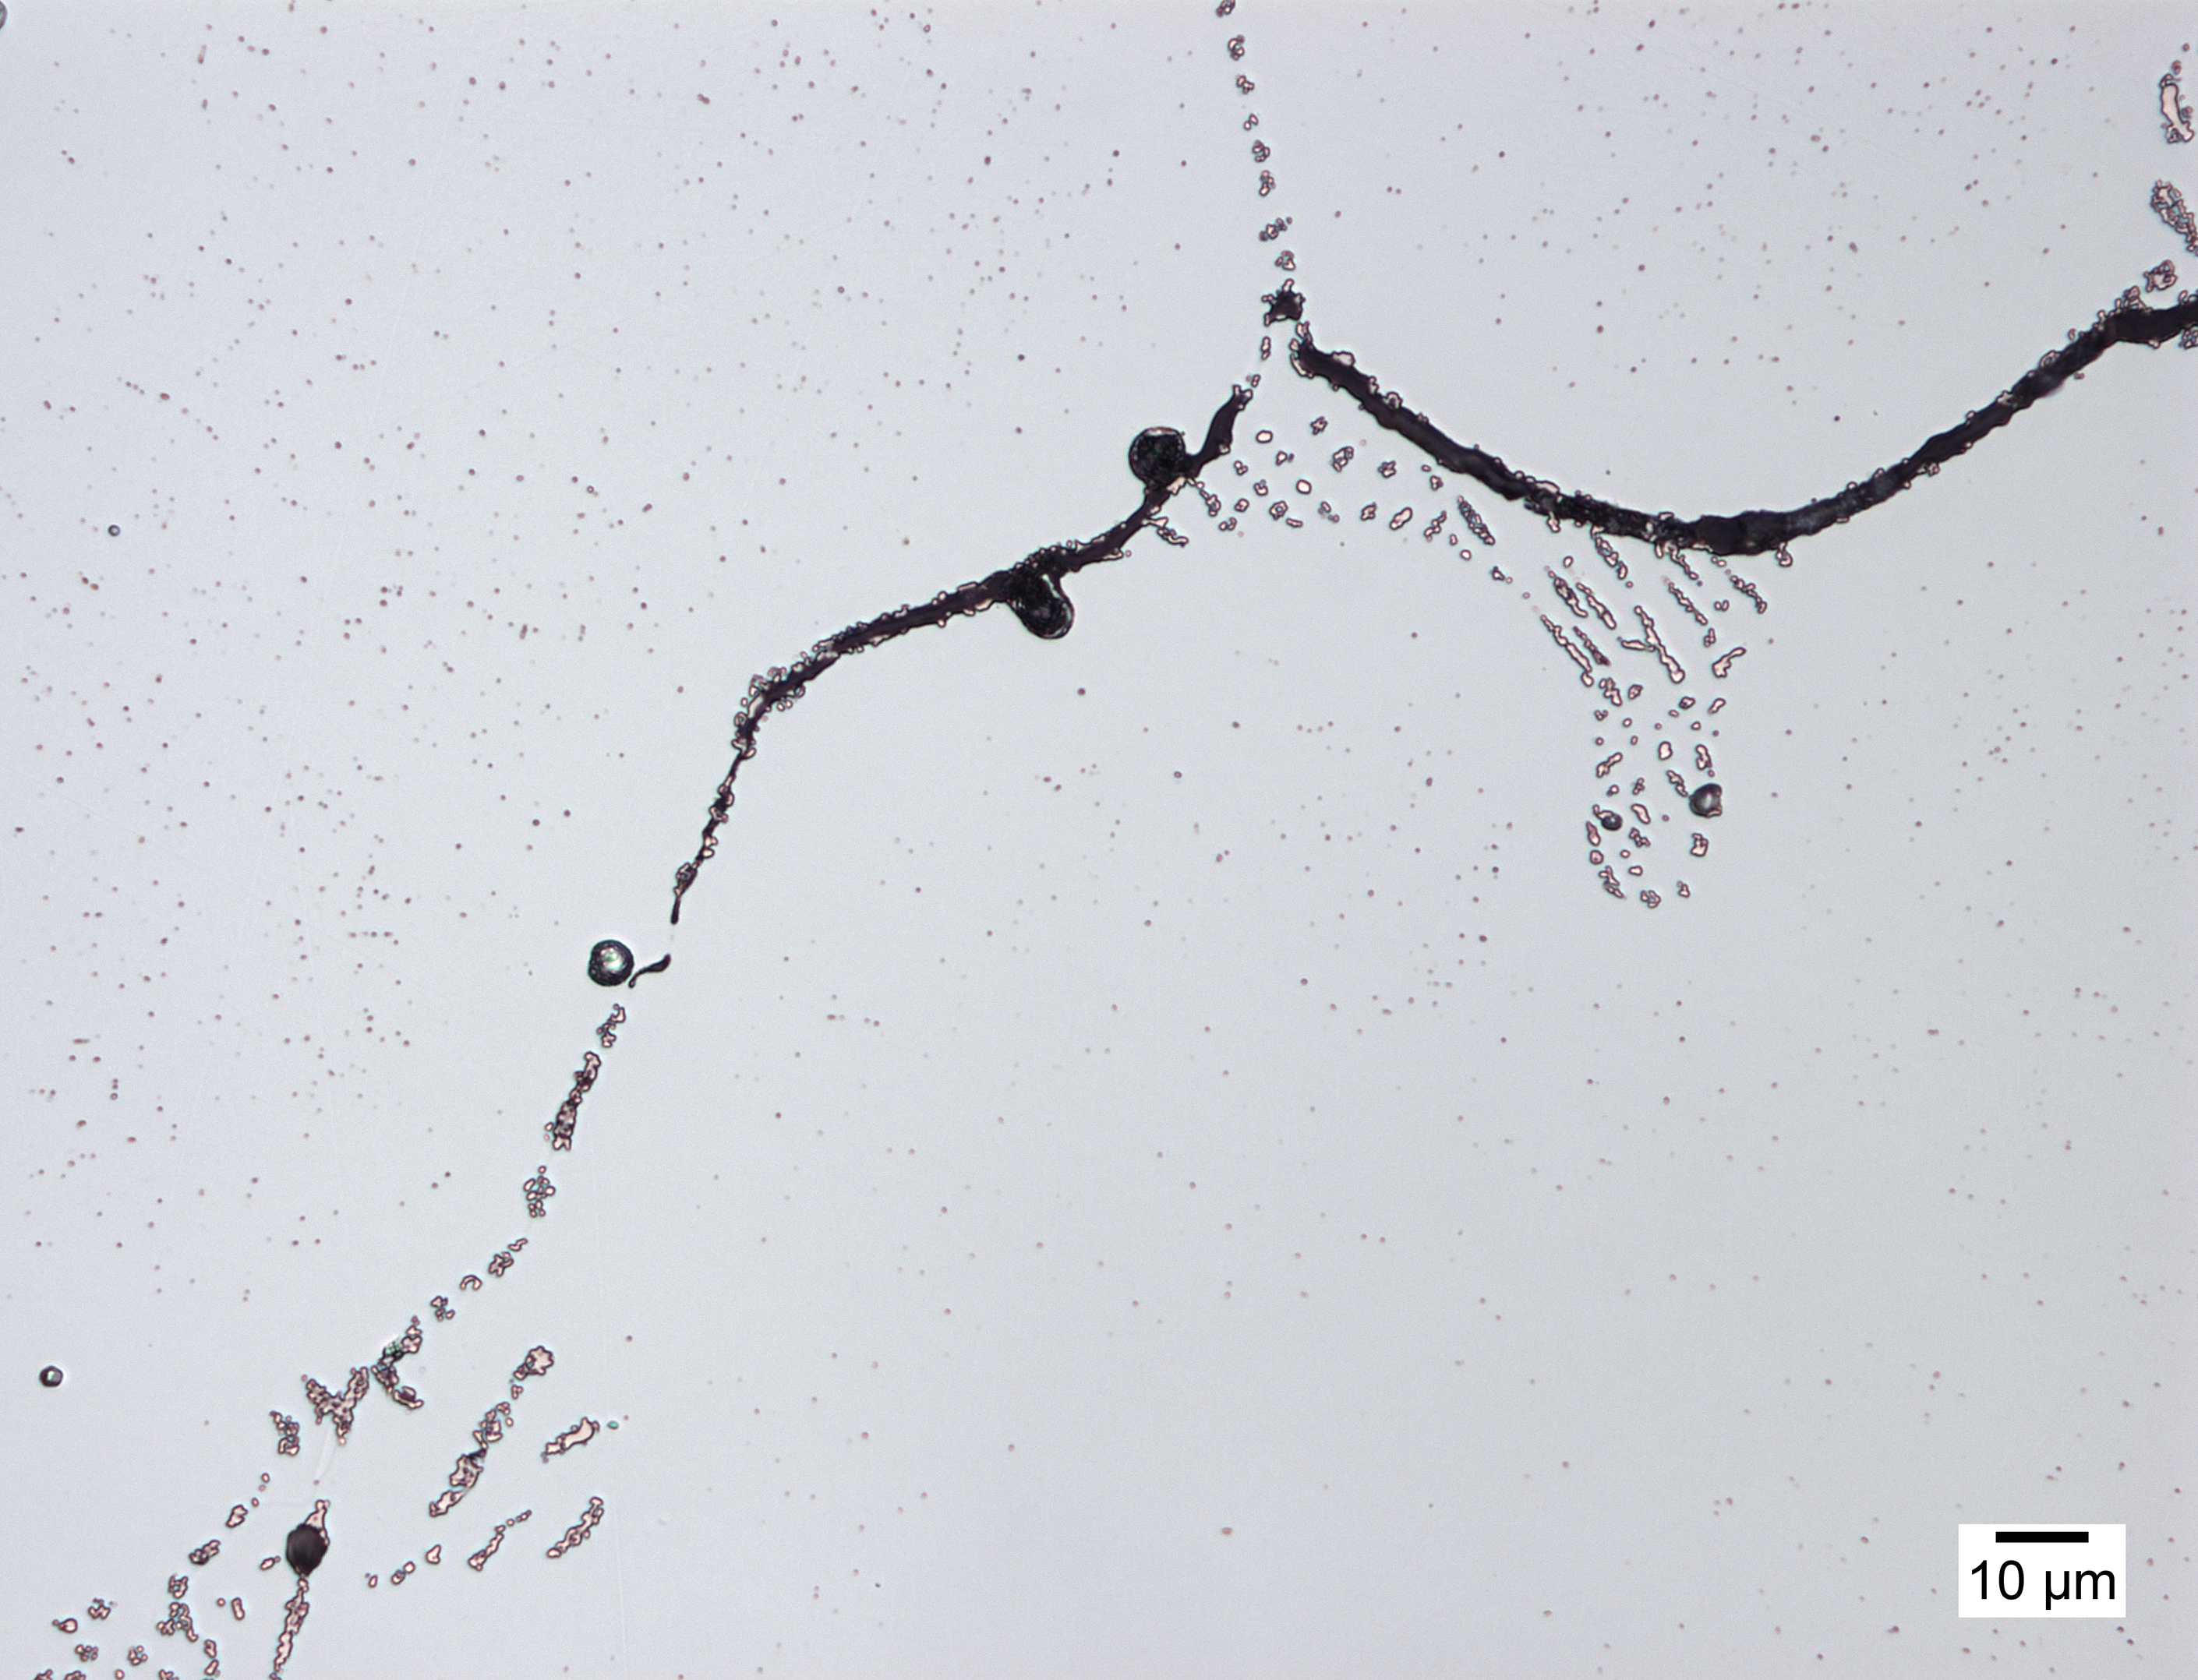
\includegraphics[width=4.7in]{figures/metallography/c5-oh-2375-narrow-crack-500x.png}}
    \caption{Optical micrographs showing wide and narrow regions at the tip of the crack visible in Figure~\ref{fig:c5-oh-2375-crack-100x}. Liquation around the interdendritic phases and on the crack faces is evident in (a), as indicated by arrows, but not in (b). Etch: electrolytic 10\% oxalic acid.}
    \label{fig:c5-oh-2375-crack-tip-500x}
\end{figure}

\begin{figure}
    \centering
    \subfloat[100X]{\label{subfig:c5-oh-2375-liquation-100x}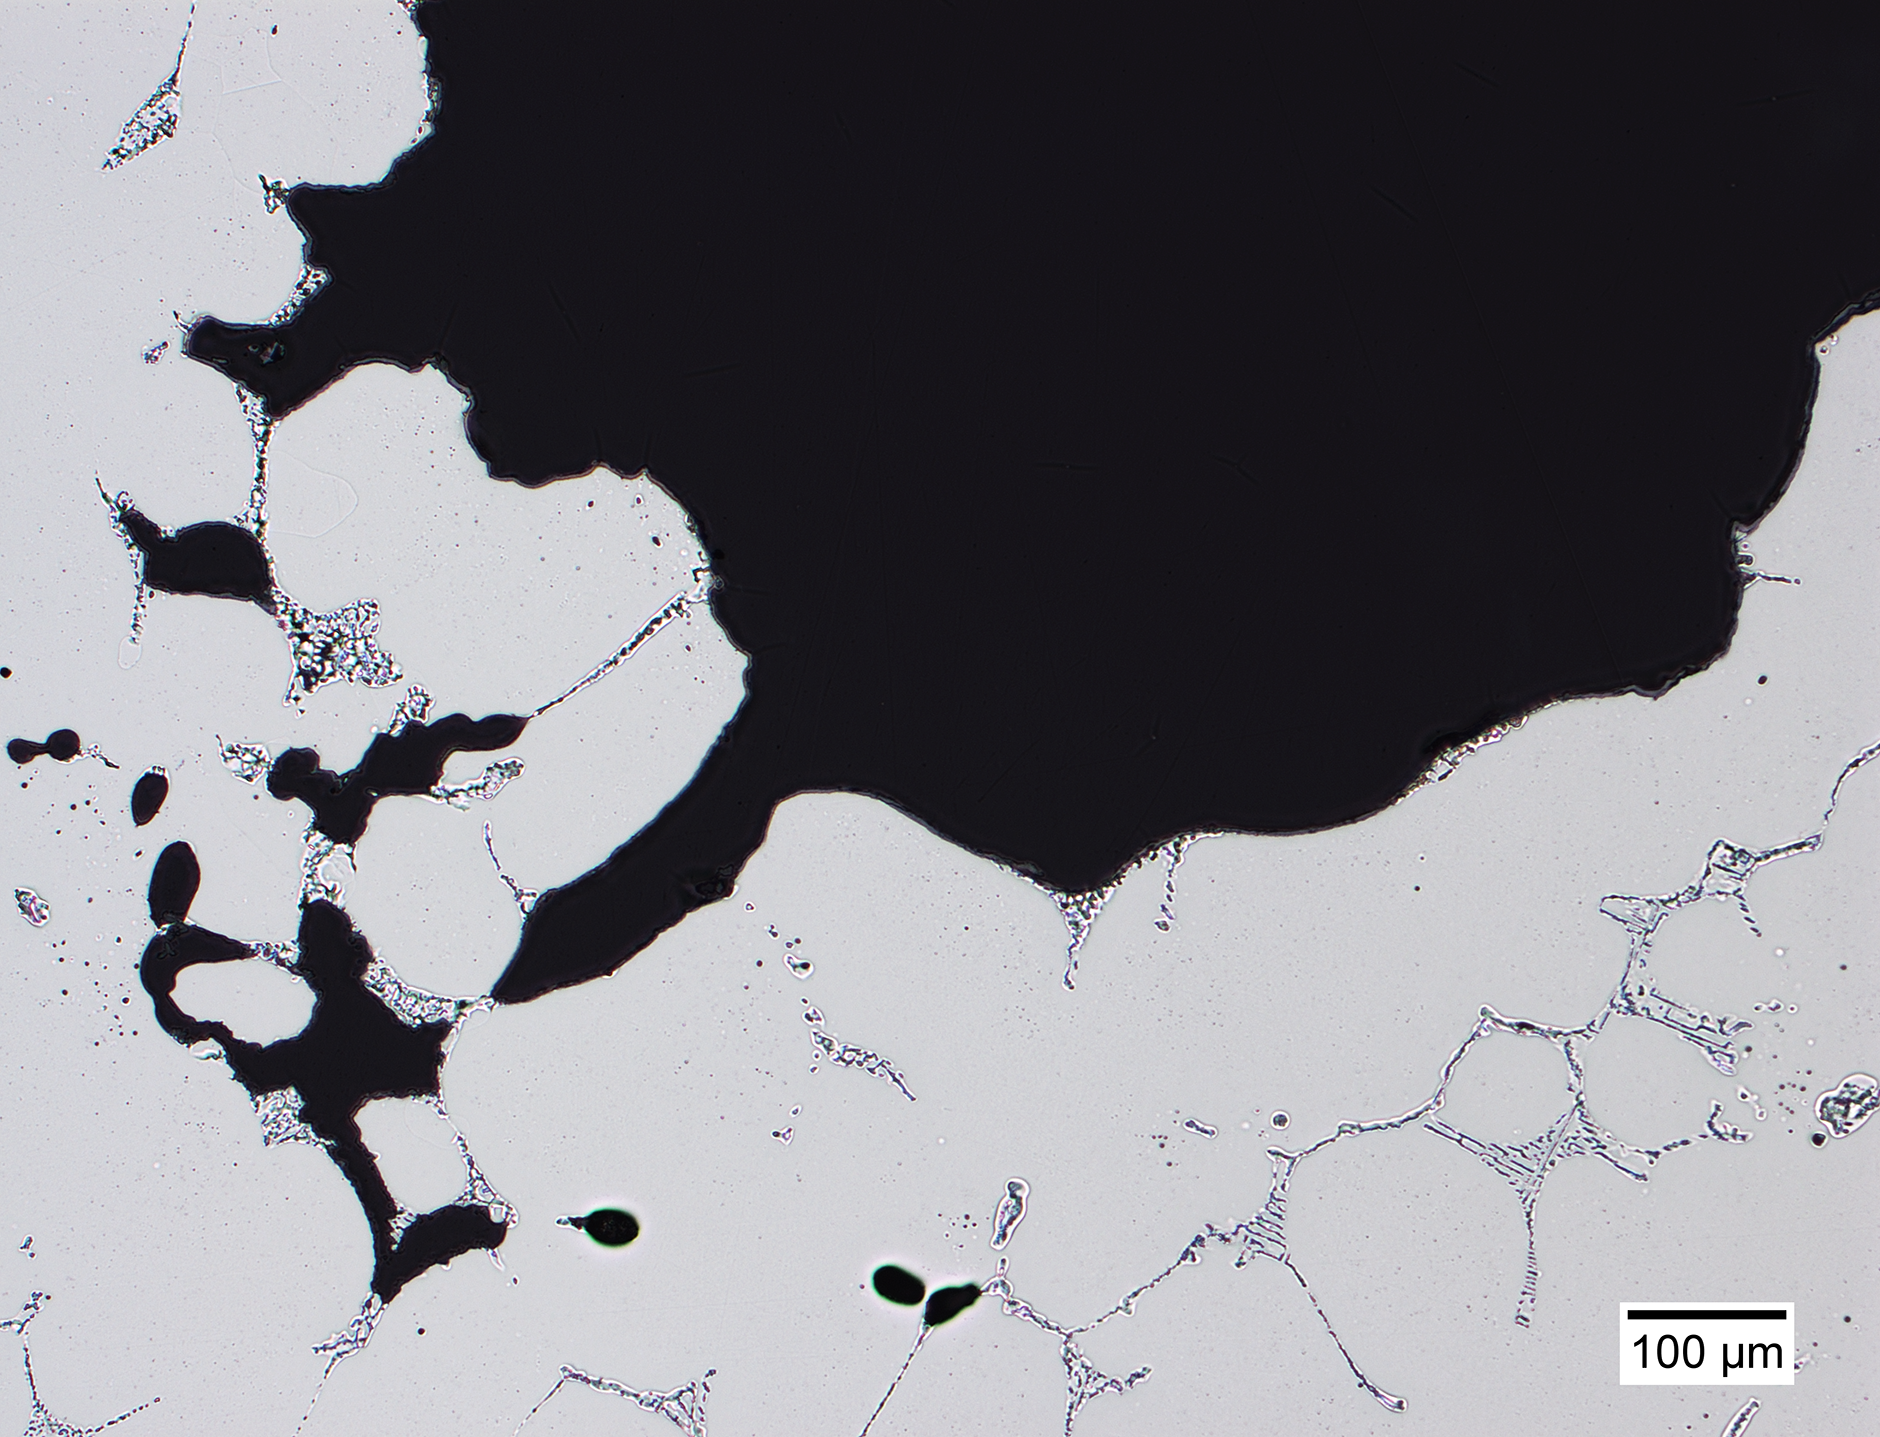
\includegraphics[width=4.7in]{figures/metallography/c5-oh-2375-liquation-100x.png}} \\
    \subfloat[500X]{\label{subfig:c5-oh-2375-liquation-500x}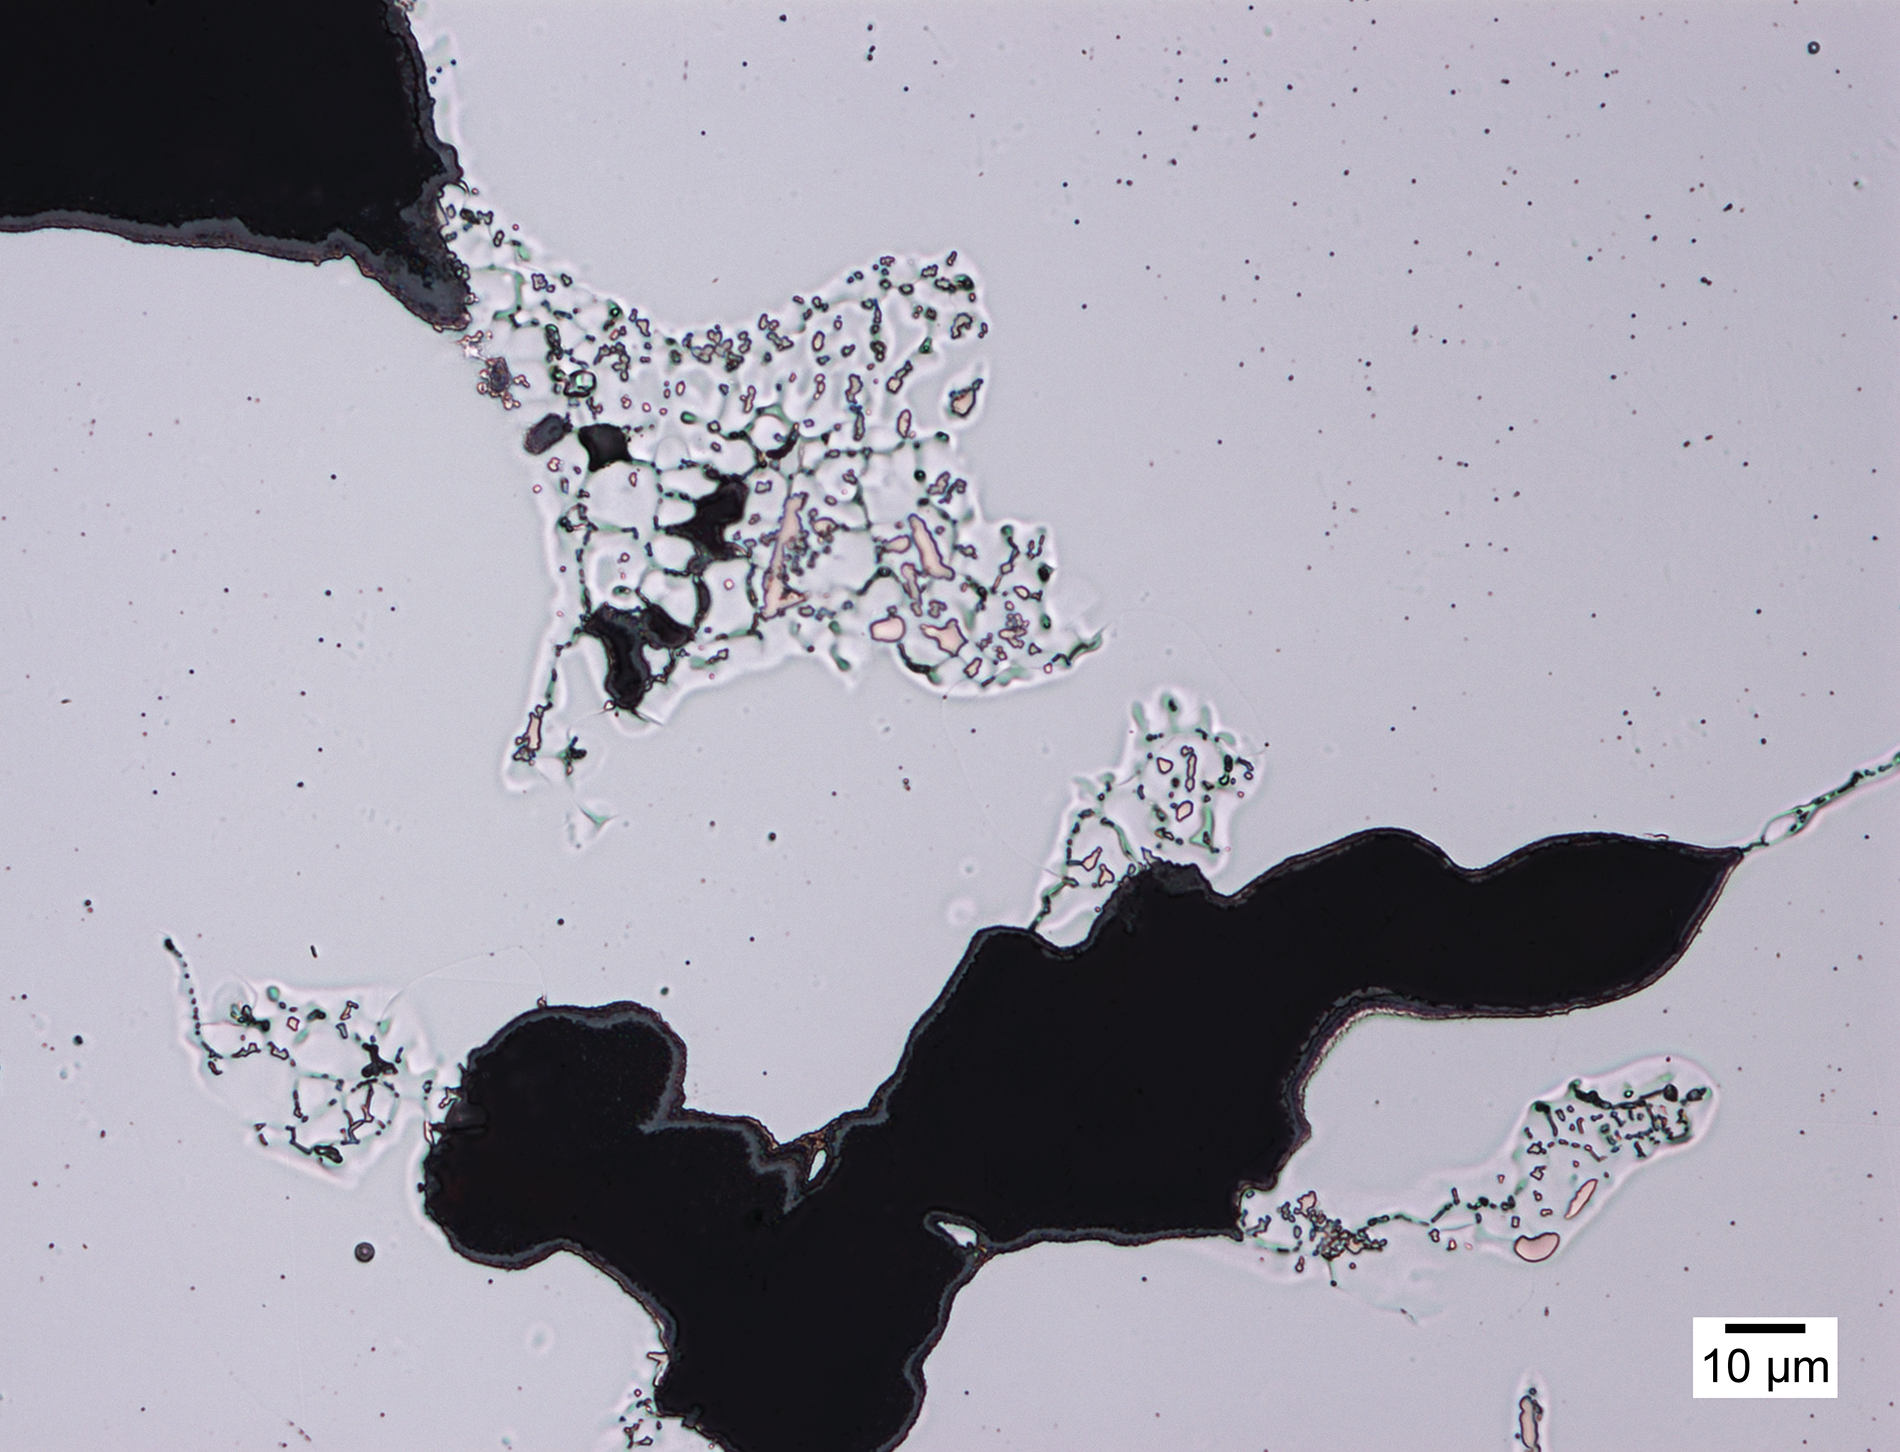
\includegraphics[width=4.7in]{figures/metallography/c5-oh-2375-liquation-500x.png}}
    \caption{Optical micrographs showing evidence of liquation around interdendritic phases near the fracture surface in the Cone~5 On-Heating 2375\textdegree{}F (C5 OH-2375) hot ductility sample. Etch: electrolytic 10\% oxalic acid.}
    \label{fig:c5-oh-2375-liquation-fracture-surface}
\end{figure}
\clearpage


\subsection{Characterization of On-Cooling Hot Ductility Tests}
\subsubsection{Cone~1 On-Cooling}
The near-surface region of the Cone~1 On-Cooling 2300F (C1 OC-2300) hot ductility sample is shown in Figure~\ref{fig:c1-oc-2300-fracture-panorama}. As with the C1 OH-2375 test (Figure~\ref{fig:c1-oh-2375}), cracking is readily apparent with the crack paths following the interdendritic boundaries, and a significant fraction of the intradendritic precipitates have dissolved. However, compared with the C1 OH-2375 sample, the C1 OC-2300 sample exhibits a much larger extent of liquid formation near the fracture surface, which is apparent in Figure~\ref{fig:c1-oc-2300-fracture-panorama} and also at higher magnification in Figure~\ref{fig:c1-oc-2300-liquation-surface} (see arrows). In these micrographs the liquid films are nearly continuous across the fracture surface. The greater extent of liquid is due to the longer duration of elevated temperature exposure for this sample, even though C1 OH-2375 and C1 OC-2300 experienced the same peak temperature (recall that the peak temperature for the on-cooling tests was chosen as the on-heating \gls{ndt}, equal to 2375\textdegree{}F). In the on-cooling tests, the sample spends a short though definite amount of time near the peak of the welding thermal cycle before being fractured on-cooling, with the precise time (1.4 s above 2360\textdegree{}F, for the thermal cycle utilized herein) dependent on the welding parameters and corresponding thermal cycle characteristics. In comparison, the on-heating \gls{ndt} sample (C1 OH-2375) was fractured immediately upon reaching the peak temperature with correspondingly less time for liquid formation.

Figure~\ref{fig:c1-oc-2300-crack-region-200x} presents a higher magnification view of the region near the tip of the crack shown in Figure~\ref{fig:c1-oc-2300-fracture-panorama}. Extensive liquated regions are apparent around the interdendritic phases and along the crack faces. The crack tip region is shown in the SEM micrographs in Figure~\ref{fig:c1-oc-2300-crack-sem}, with the corresponding EDS analysis results (from the box in Figure~\ref{subfig:c1-oc-2300-crack-5kx}) given in Figure~\ref{fig:c1-oc-2300-crack-tip-particles-eds}. There are numerous small particles located on the crack faces and on the interdendritic boundary ahead of the crack tip, which are enriched in Nb (Figure~\ref{fig:c1-oc-2300-crack-tip-particles-eds}); the Fe, Cr, and Ni peaks most likely originate from the surrounding matrix. Notably, Si enrichment above the nominal alloy composition is not observed which indicates the Ni-Nb-Si silicide phase is not present in the interdendritic region depicted here. 

The liquated region surrounding some of the interdendritic phases in Figure~\ref{fig:c1-oc-2300-fracture-panorama} is evaluated further in the SEM micrographs in Figure~\ref{fig:c1-oc-2300-sem-liquid} with corresponding EDS spot analysis results in Figure~\ref{fig:c1-oc-2300-liquid-eds}. The quantitative EDS results indicate that the white particle is NbC while the surrounding liquid (around the interdendritic phases) is essentially similar to the nominal alloy composition and is not enriched in Ni, Nb, or Si. This fact suggests that the formation of liquid in this region (along the interdendritic boundaries) is not due to melting of Ni-Nb-Si phases during the simulated on-cooling thermal cycle. [add possible explanations for formation of liquid that are not due to melting of low Tm phases].

%C1 On-cooling figures
\begin{landscape}
\begin{figure}
    \centering
    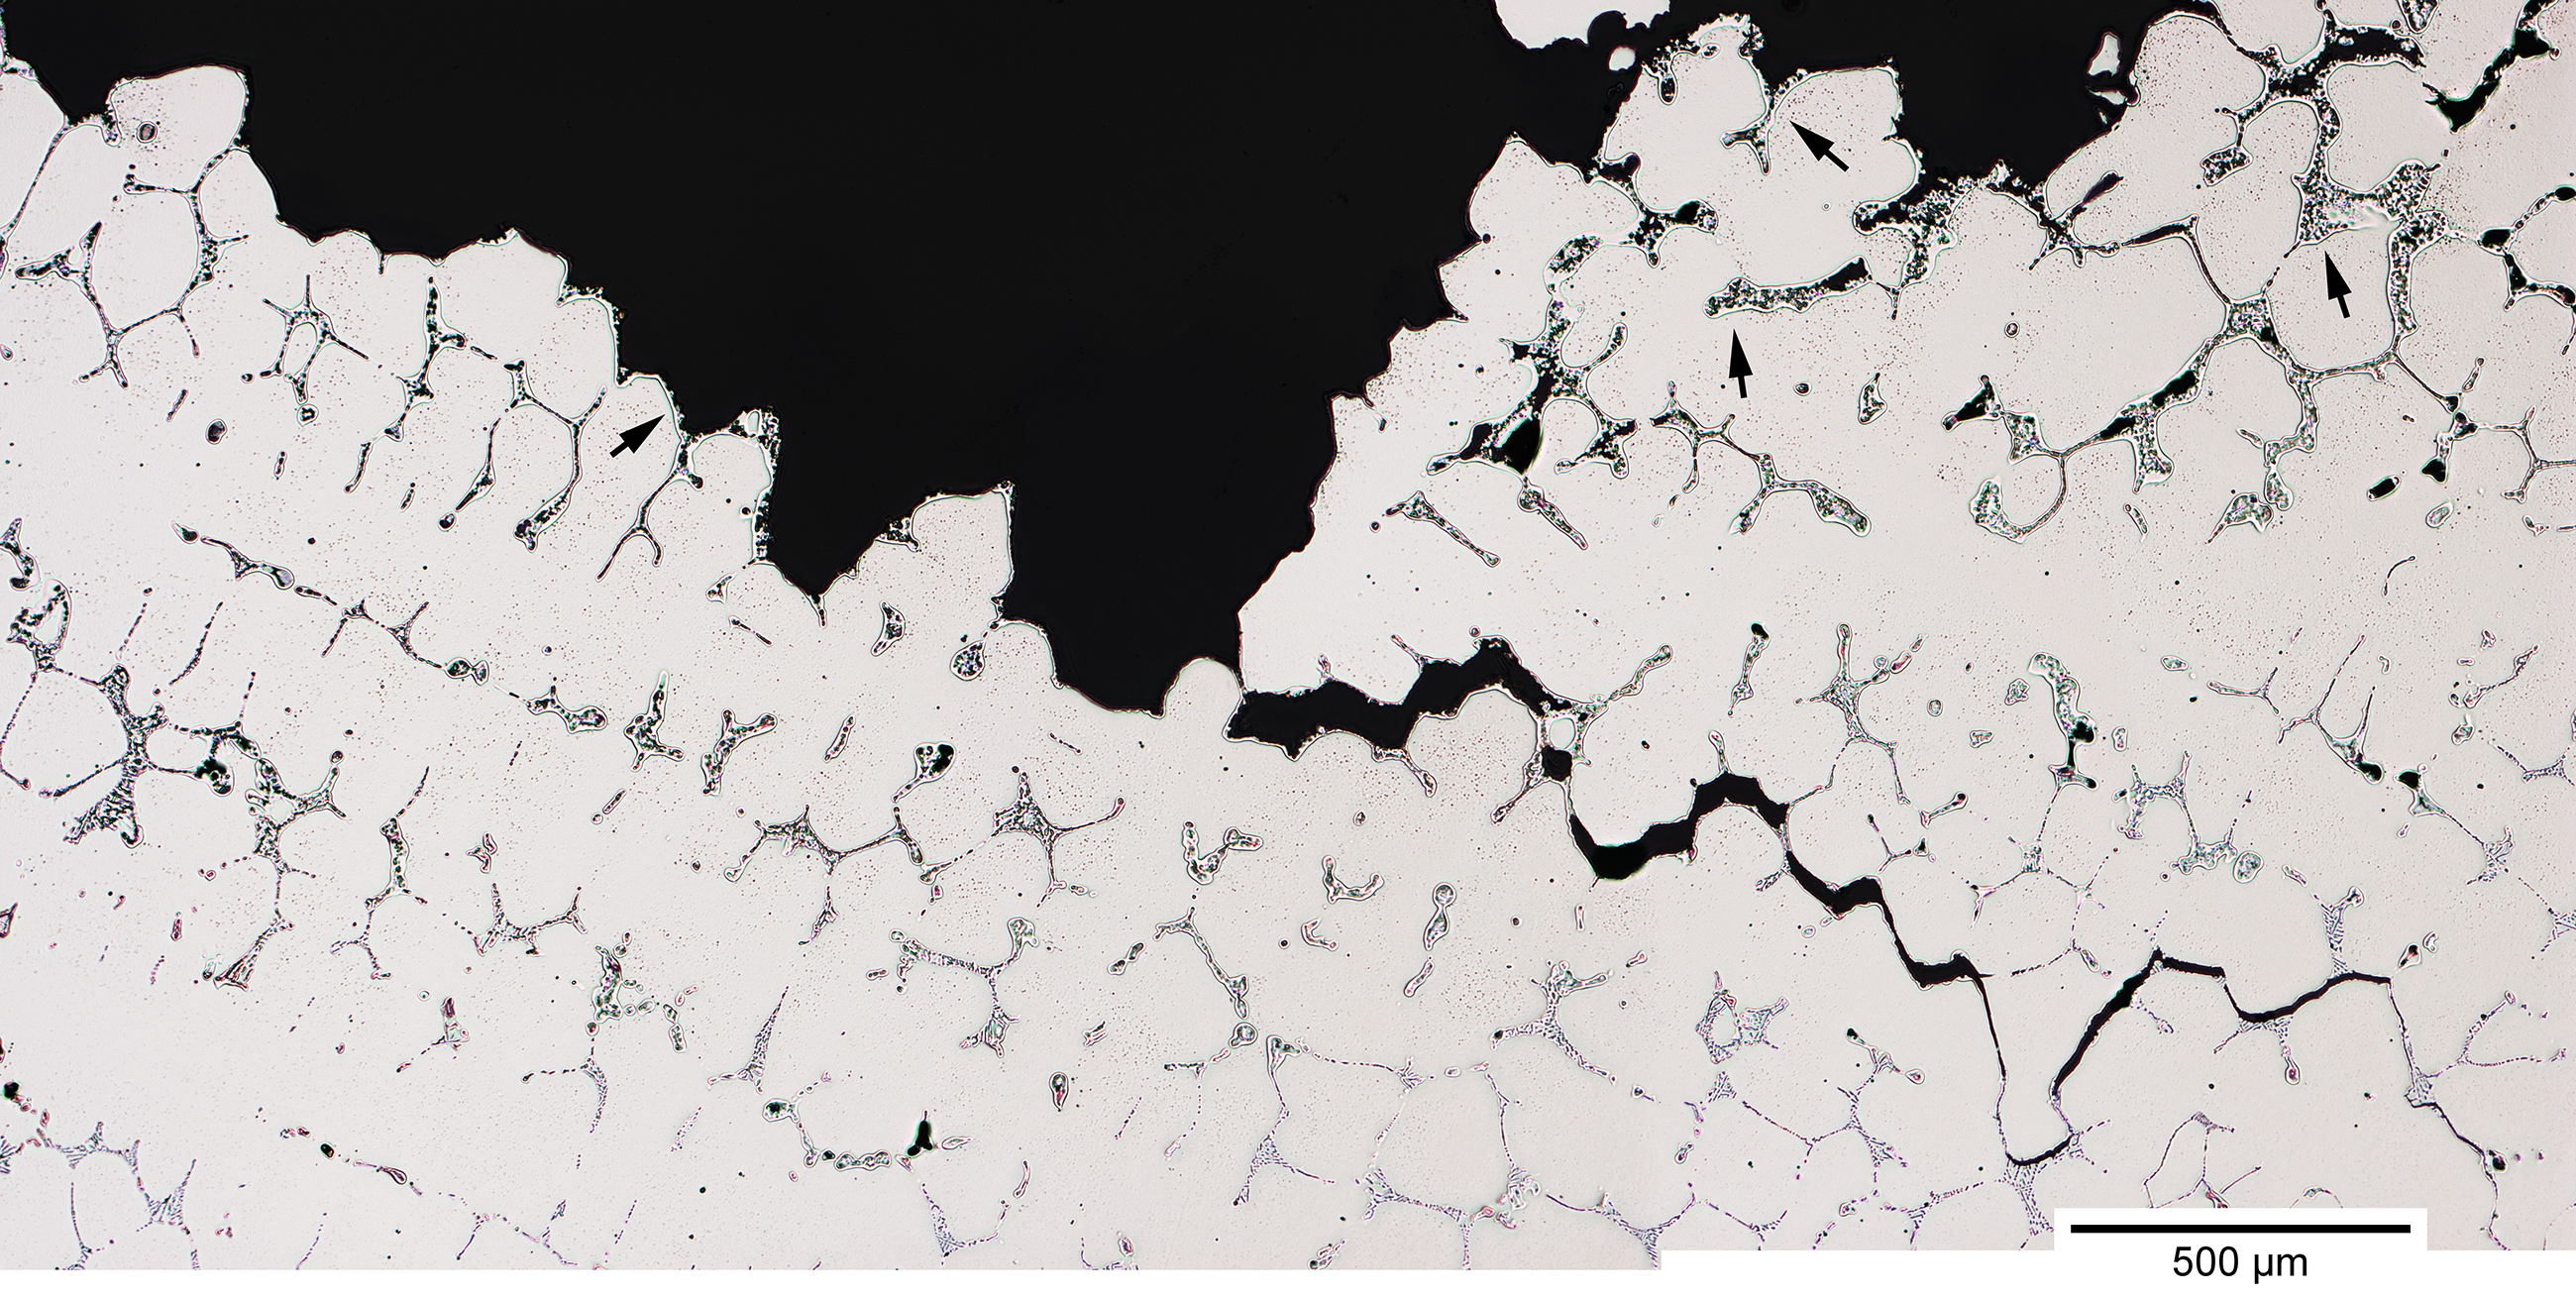
\includegraphics[width=8in]{figures/metallography/c1-oc-2300-fracture-panorama.png}
    \caption{Optical micrograph of a region of the fracture surface in the Cone~1 On-Cooling 2300\textdegree{}F (C1 OC-2300) hot ductility sample. Note the extensive formation of liquated regions near the surface (e.g. as denoted by arrows). Original magnification, 50X. Etch: electrolytic 10\% oxalic acid.}
    \label{fig:c1-oc-2300-fracture-panorama}
\end{figure}
\end{landscape}

\begin{figure}
    \centering
    \includegraphics[width=4.7in]{figures/metallography/c1-oc-2300-liquation-surface-100x.png}
    \caption{Optical micrograph showing a nearly continuous liquid film (arrows) along the fracture surface of the Cone~1 On-Cooling 2300\textdegree{}F (C1 OC-2300) hot ductility sample, 100X. Etch: electrolytic 10\% oxalic acid.}
    \label{fig:c1-oc-2300-liquation-surface}
\end{figure}

\begin{figure}
    \centering
    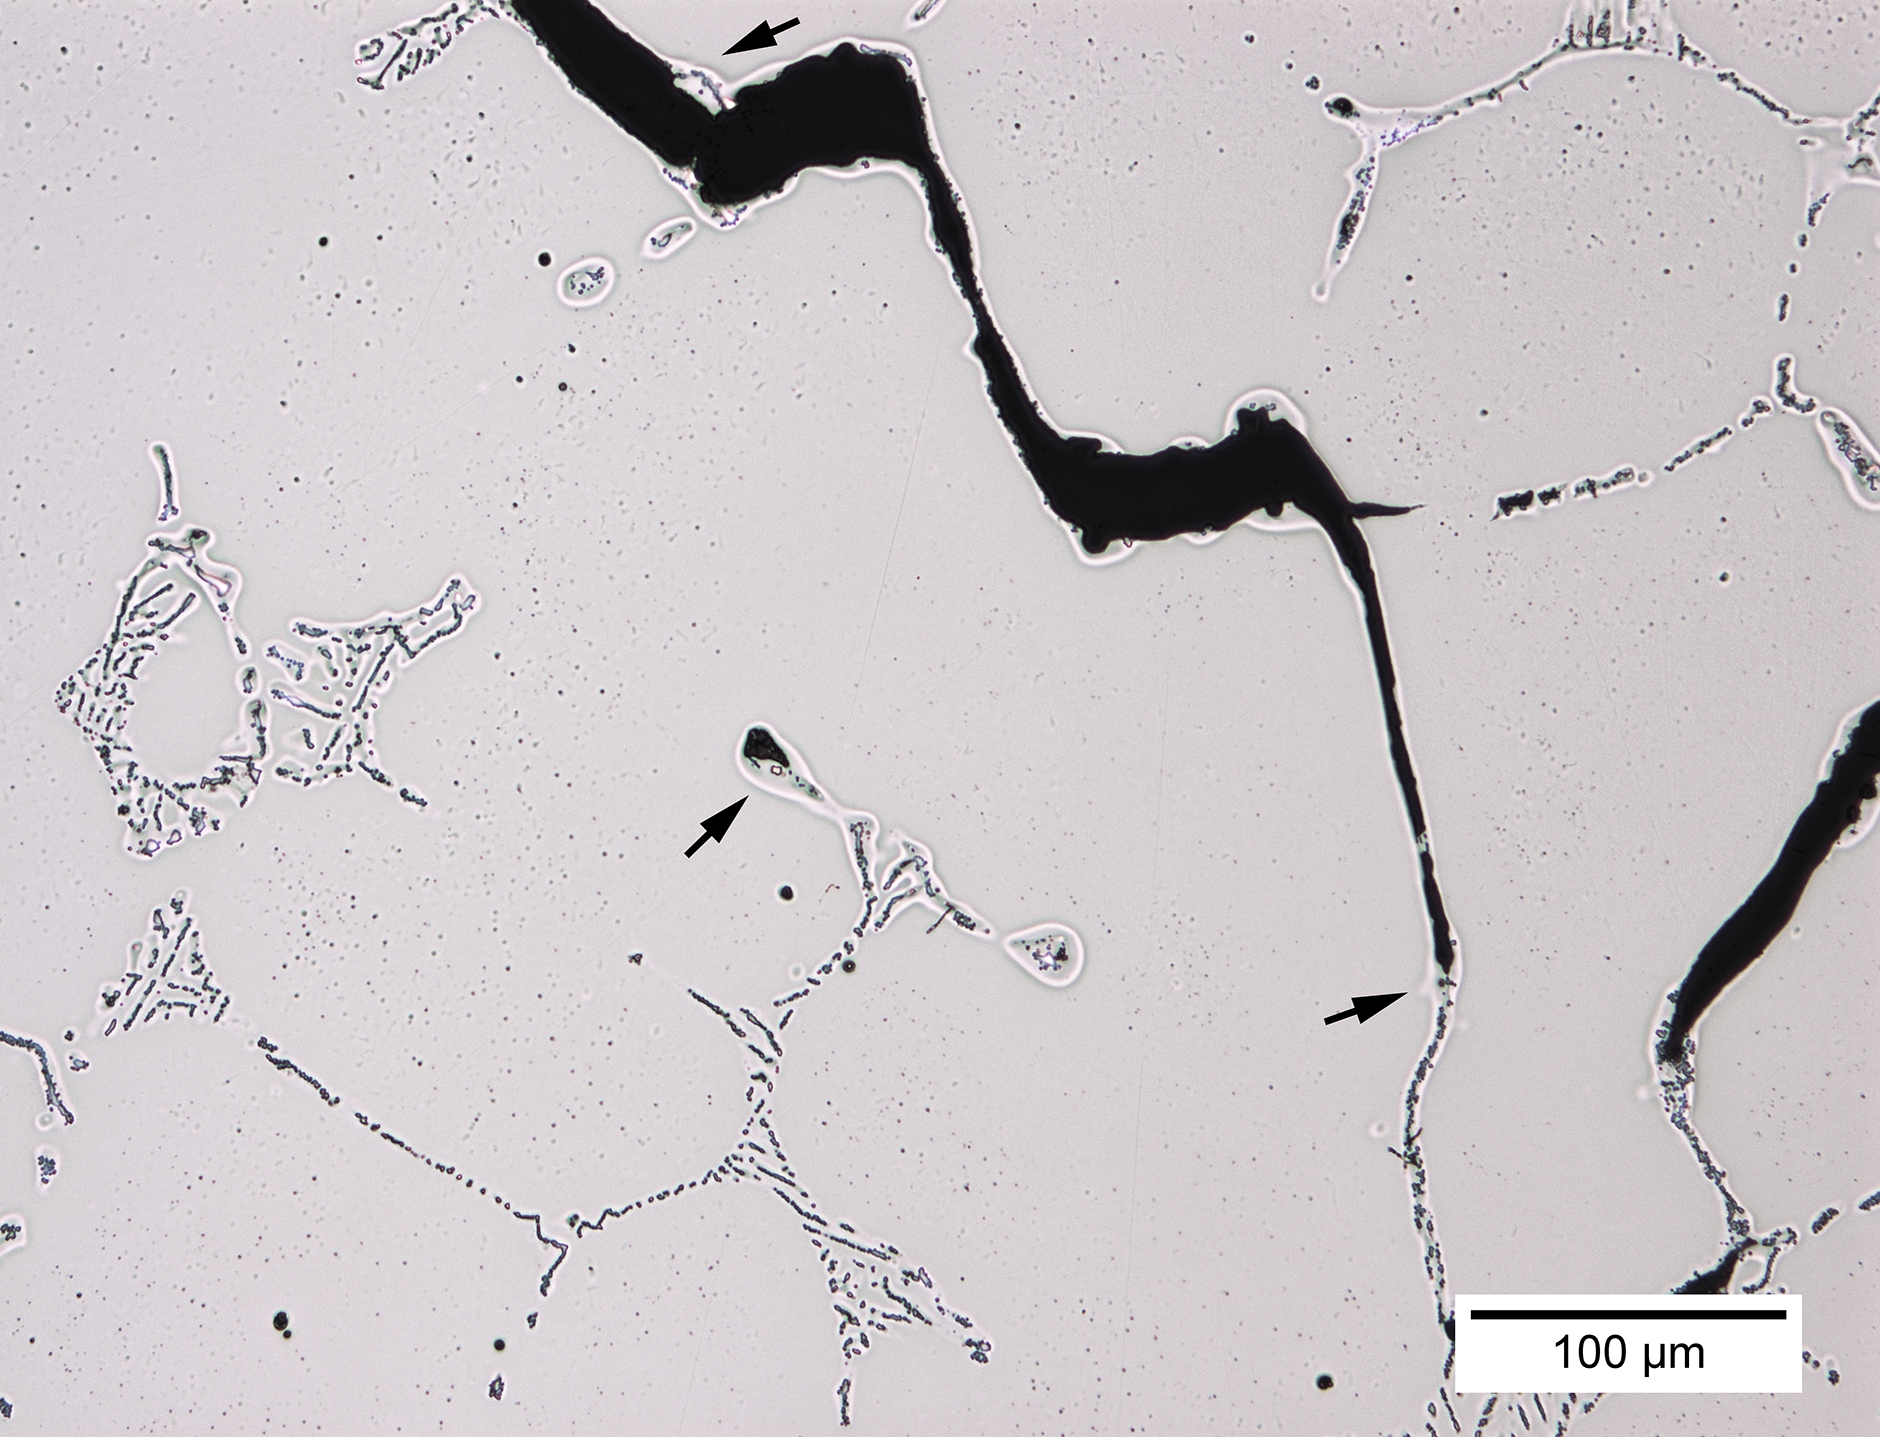
\includegraphics[width=4.7in]{figures/metallography/c1-oc-2300-crack-region-200x.png}
    \caption[]{Optical micrograph showing extensive liquation (arrows) along the crack faces and surrounding interdendritic phases, near the tip of the crack visible in Figure~\ref{fig:c1-oc-2300-fracture-panorama} for the Cone~1 On-Cooling 2300\textdegree{}F (C1 OC-2300) hot ductility sample, 200X. Etch: electrolytic 10\% oxalic acid.}
    \label{fig:c1-oc-2300-crack-region-200x}
\end{figure}

\begin{figure}
    \centering
    \subfloat[1000X]{\label{subfig:c1-oc-2300-crack-1kx}\includegraphics[width=4.7in]{figures/metallography/c1-oc-2300-crack-1kx-L3-17.png}} \\
    \subfloat[5000X]{\label{subfig:c1-oc-2300-crack-5kx}\includegraphics[width=4.7in]{figures/metallography/c1-oc-2300-crack-5kx-L3-19.png}}
    \caption{\Gls{sem} micrographs showing the region at the tip of the crack visible in Figure~\ref{fig:c1-oc-2300-fracture-panorama} for the Cone~5 On-Heating 2375\textdegree{}F (C5 OH-2375) hot ductility sample. The \gls{eds} results for the boxed area in (b) are given in Figure~\ref{fig:c1-oc-2300-crack-tip-particles-eds}. Etch: electrolytic 10\% oxalic acid.}
    \label{fig:c1-oc-2300-crack-sem}
\end{figure}

\begin{figure}
    \centering
    \includegraphics[width=\textwidth]{figures/metallography/c1-oc-2300-crack-tip-particles-eds-table.png}
    \caption{\Gls{eds} results for the boxed area shown in Figure~\ref{subfig:c1-oc-2300-crack-5kx}, at the tip of the crack.}
    \label{fig:c1-oc-2300-crack-tip-particles-eds}
\end{figure}


\begin{figure}
    \centering
    \subfloat[1000X]{\label{subfig:c1-oc-2300-sem-liquid-1kx}\includegraphics[width=4.7in]{figures/metallography/c1-oc-2300-liquid-L1-1kx-01.png}} \\
    \subfloat[5000X]{\label{subfig:c1-oc-2300-sem-liquid-5kx}\includegraphics[width=4.7in]{figures/metallography/c1-oc-2300-liquid-L1-5kx-04.png}}
    \caption[]{\Gls{sem} micrographs showing evidence of liquation around interdendritic phases adjacent to the fracture surface in the Cone~1 On-Cooling 2300\textdegree{}F hot ductility sample. \Gls{eds} spot analysis results for the indicated points ``A'' and ``B'' in (b) are given in Figure~\ref{fig:c1-oc-2300-liquid-eds}.}
    \label{fig:c1-oc-2300-sem-liquid}
\end{figure}

\begin{figure}
    \centering
    \subfloat[Spot \gls{eds} results for point ``A'']{\label{subfig:c1-oc-2300-liquid-eds-A}\includegraphics[width=\textwidth]{figures/metallography/c1-oc-2300-liquid-eds-table-A.png}} \\
    \subfloat[Spot \gls{eds} results for point ``B'']{\label{subfig:c1-oc-2300-liquid-eds-B}\includegraphics[width=\textwidth]{figures/metallography/c1-oc-2300-liquid-eds-table-B.png}}
    \caption{Spot \gls{eds} results for the indicated points ``A'' and ``B'' in Figure~\ref{subfig:c1-oc-2300-sem-liquid-5kx} for the Cone~1 On-Cooling 2300\textdegree{}F (C1 OC-2300) hot ductility sample.}
    \label{fig:c1-oc-2300-liquid-eds}
\end{figure}
\clearpage

\subsubsection{Cone~5 On-Cooling}
Figure~\ref{fig:c5-oc-2300-fracture-50x} shows a region adjacent to the fracture surface of the Cone~5 On-Cooling 2300\textdegree{}F (C5 OC-2300) hot ductility sample. As with the C1 OC-2300 sample, C5 OC-2300 shows significant cracking along the interdendritic boundaries (with the cracked boundaries generally oriented perpendicular to the tensile loading direction). Extensive liquation is also apparent in Figure~\ref{fig:c5-oc-2300-fracture-50x}, both along the edge of the fracture profile and around the interdendritic phases slightly away from fracture. The extent of liquid formed is similar to the C1 OC-2300 sample and as in that case, the greater extent of liquid formation compared to the on-heating test (C5 OH-2375) is due to the longer exposure to the peak temperature of simulated thermal cycle. The tip of the larger crack from Figure~\ref{fig:c5-oc-2300-fracture-50x} is shown at higher magnification in Figure~\ref{fig:c5-oc-2300-crack-olm}, where liquation is evident around the interdendritic boundary ahead of the crack as well as nearby secondary phases (denoted by arrows). The tip of the crack was examined in the \gls{sem} as shown in Figure~\ref{fig:c5-oc-2300-crack-tip-sem}. The compositions of the indicated points in Figure~\ref{subfig:c5-oc-2300-crack-sem-5kx}, corresponding to the liquated region around the crack and a nearby particle, are shown in Figure~\ref{fig:c5-oc-2300-crack-tip-eds} as determined by \gls{eds}. The liquated region near the crack tip shows essentially the nominal alloy composition and does not reveal Ni, Nb, or Si enrichment, while the particle (whitish in appearance) is shown to enriched in Nb (29 wt.\%) and thus most likely a niobium carbide, with other peaks (near the nominal alloy composition) in the spectrum from the surrounding matrix.

Another liquated region near the fracture surface is shown in the optical micrographs in Figure~\ref{fig:c5-oc-2300-liquation-olm}. A significant extent of liquid formation is evident surrounding a region with eutectic-like structure. The boxed region in Figure~\ref{subfig:c5-oc-2300-liquation-500x} is examined at higher magnification in the SEM micrographs (using back-scattered electron \gls{bse} imaging mode) presented in Figure~\ref{fig:c5-oc-2300-liquation-sem}. The \gls{eds} results for the three indicated points are given in Figure~\ref{fig:c5-oc-2300-liquation-eds}. Point ``A'' corresponds to the liquid and shows a composition close to the nominal alloy composition, but with a slight enrichment in Si and Mn (2.4 wt.\% and 2 wt.\% respectively). It is apparent from Figure~\ref{subfig:c5-oc-2300-crack-sem-5kx} that the phases (highlighted by arrows) at points ``B'' and ``C'' have a different appearance from the surrounding brighter ``white''-appearing particles (which are NbC), resulting from the chemical composition contrast provided by \gls{bse} imaging. Both phases analyzed at points ``B'' and ``C'' are enriched in Si, Ni, and Nb compared to the nominal alloy composition. However, the \gls{eds} compositions are not close to that of G-phase (Ni16Nb6Si7) which has a composition of 55.8 wt.\% Ni, 32.9 wt.\% Nb, and 11.6 wt.\% Si \cite{hoffman_high_2000-1}.

%Ni-Nb-Si enriched phases were found only rarely, and the liquid observed in both on-heating and on-cooling tests was not found to be enriched in these elements

% Patchett suggested that the liquation cracking mechanism follows a Thompson constitutional liquation model with NbC and a Si-Ni phase

\begin{figure}
    \centering
    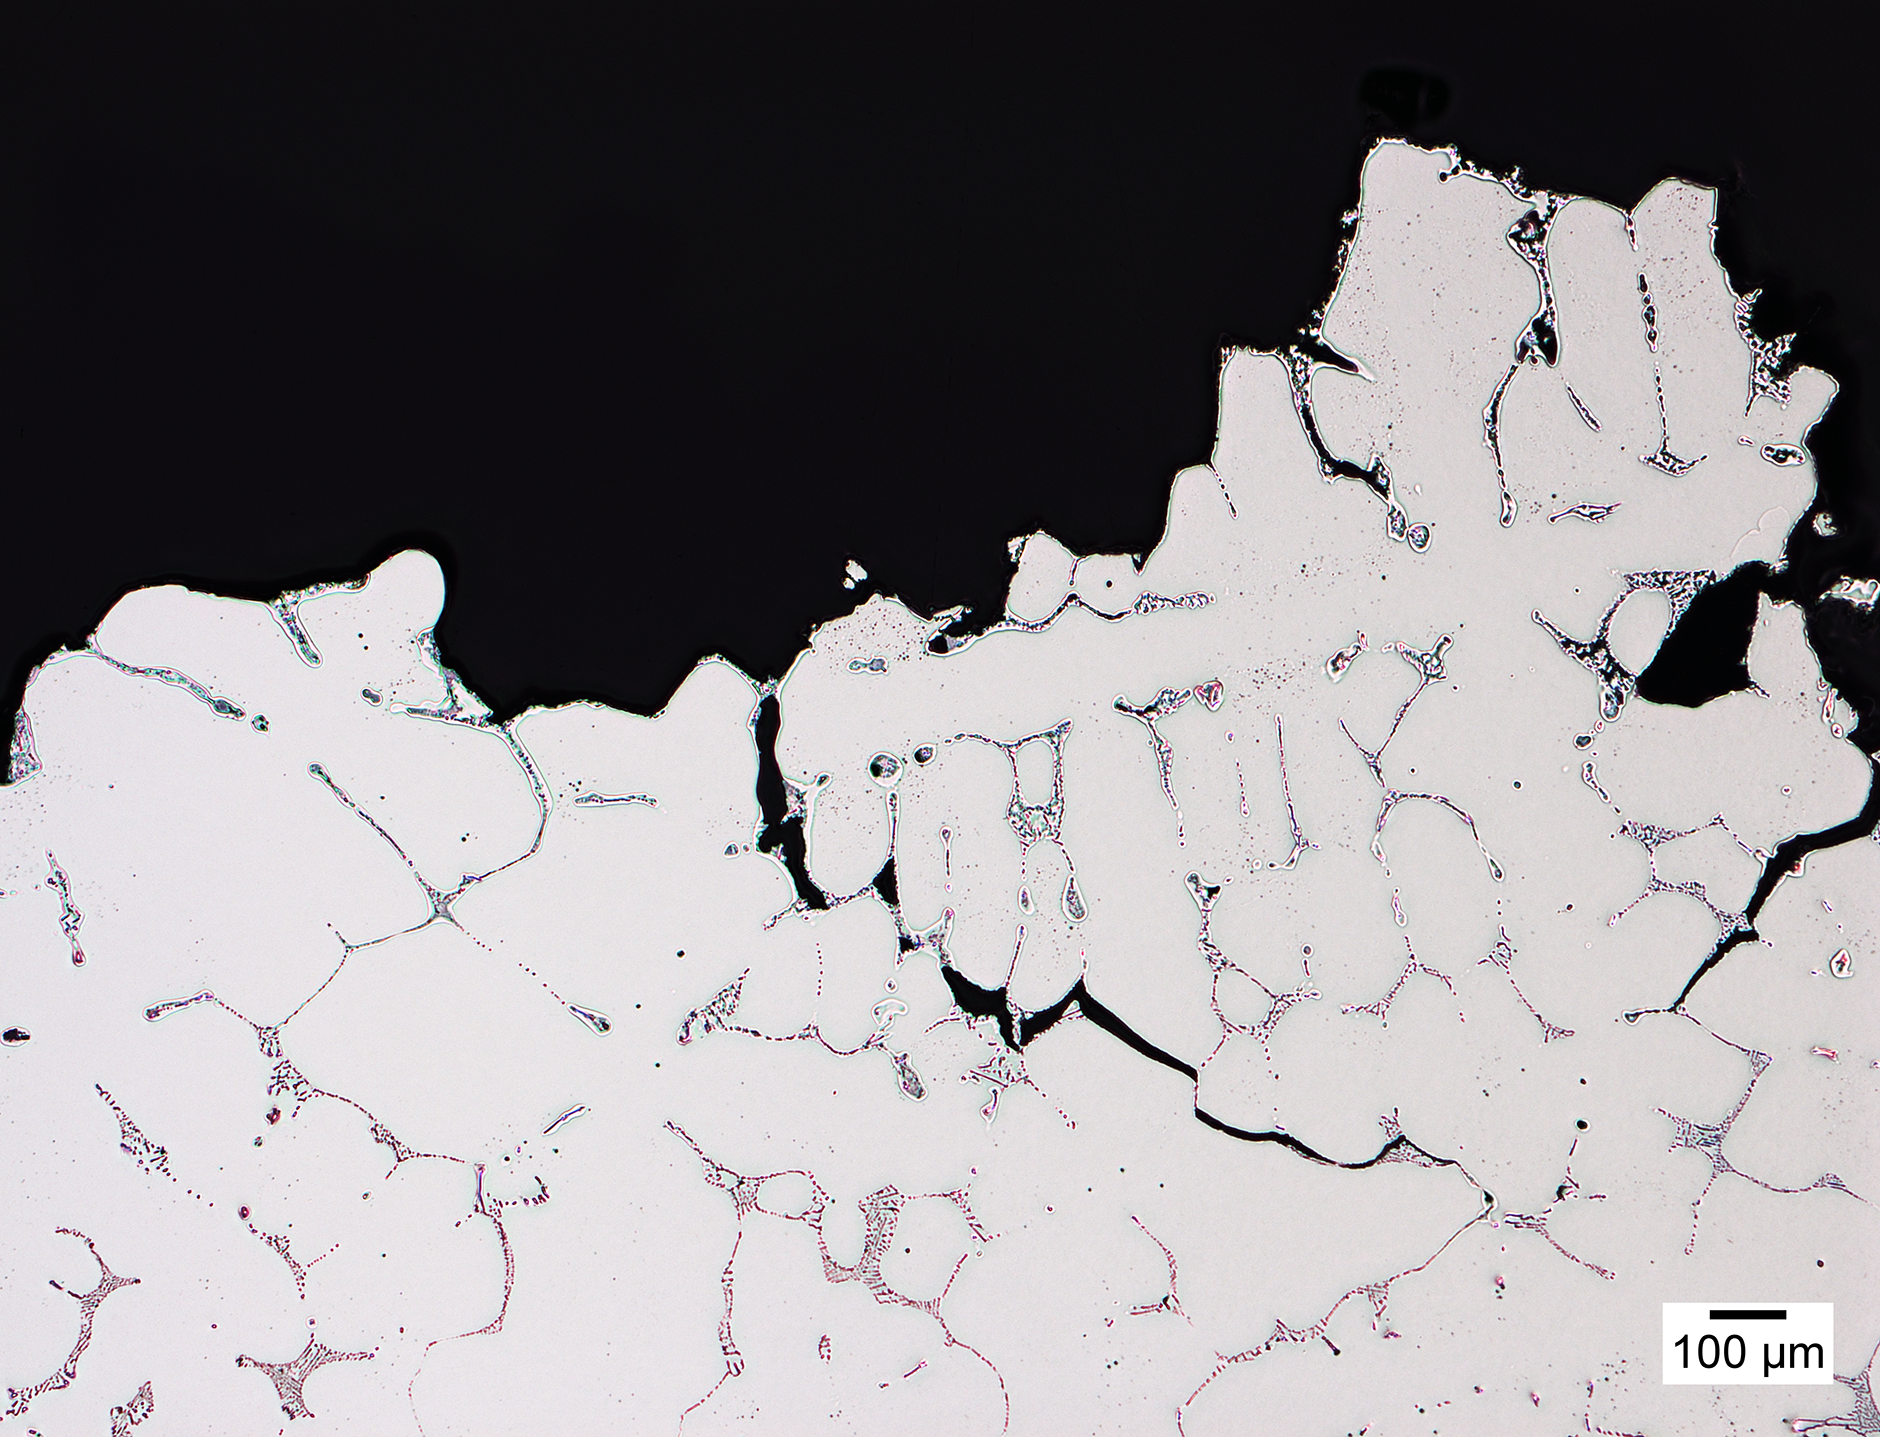
\includegraphics[width=4.7in]{figures/metallography/c5-oc-2300-fracture-50x.png}
    \caption{Optical micrograph showing a region adjacent to the fracture surface in the Cone~5 On-Cooling 2300\textdegree{}F (C5 OC-2300) hot ductility sample. Etch: electrolytic 10\% oxalic acid.}
    \label{fig:c5-oc-2300-fracture-50x}
\end{figure}

\begin{figure}
    \centering
    \subfloat[100X]{\label{subfig:c5-oc-2300-crack-100x}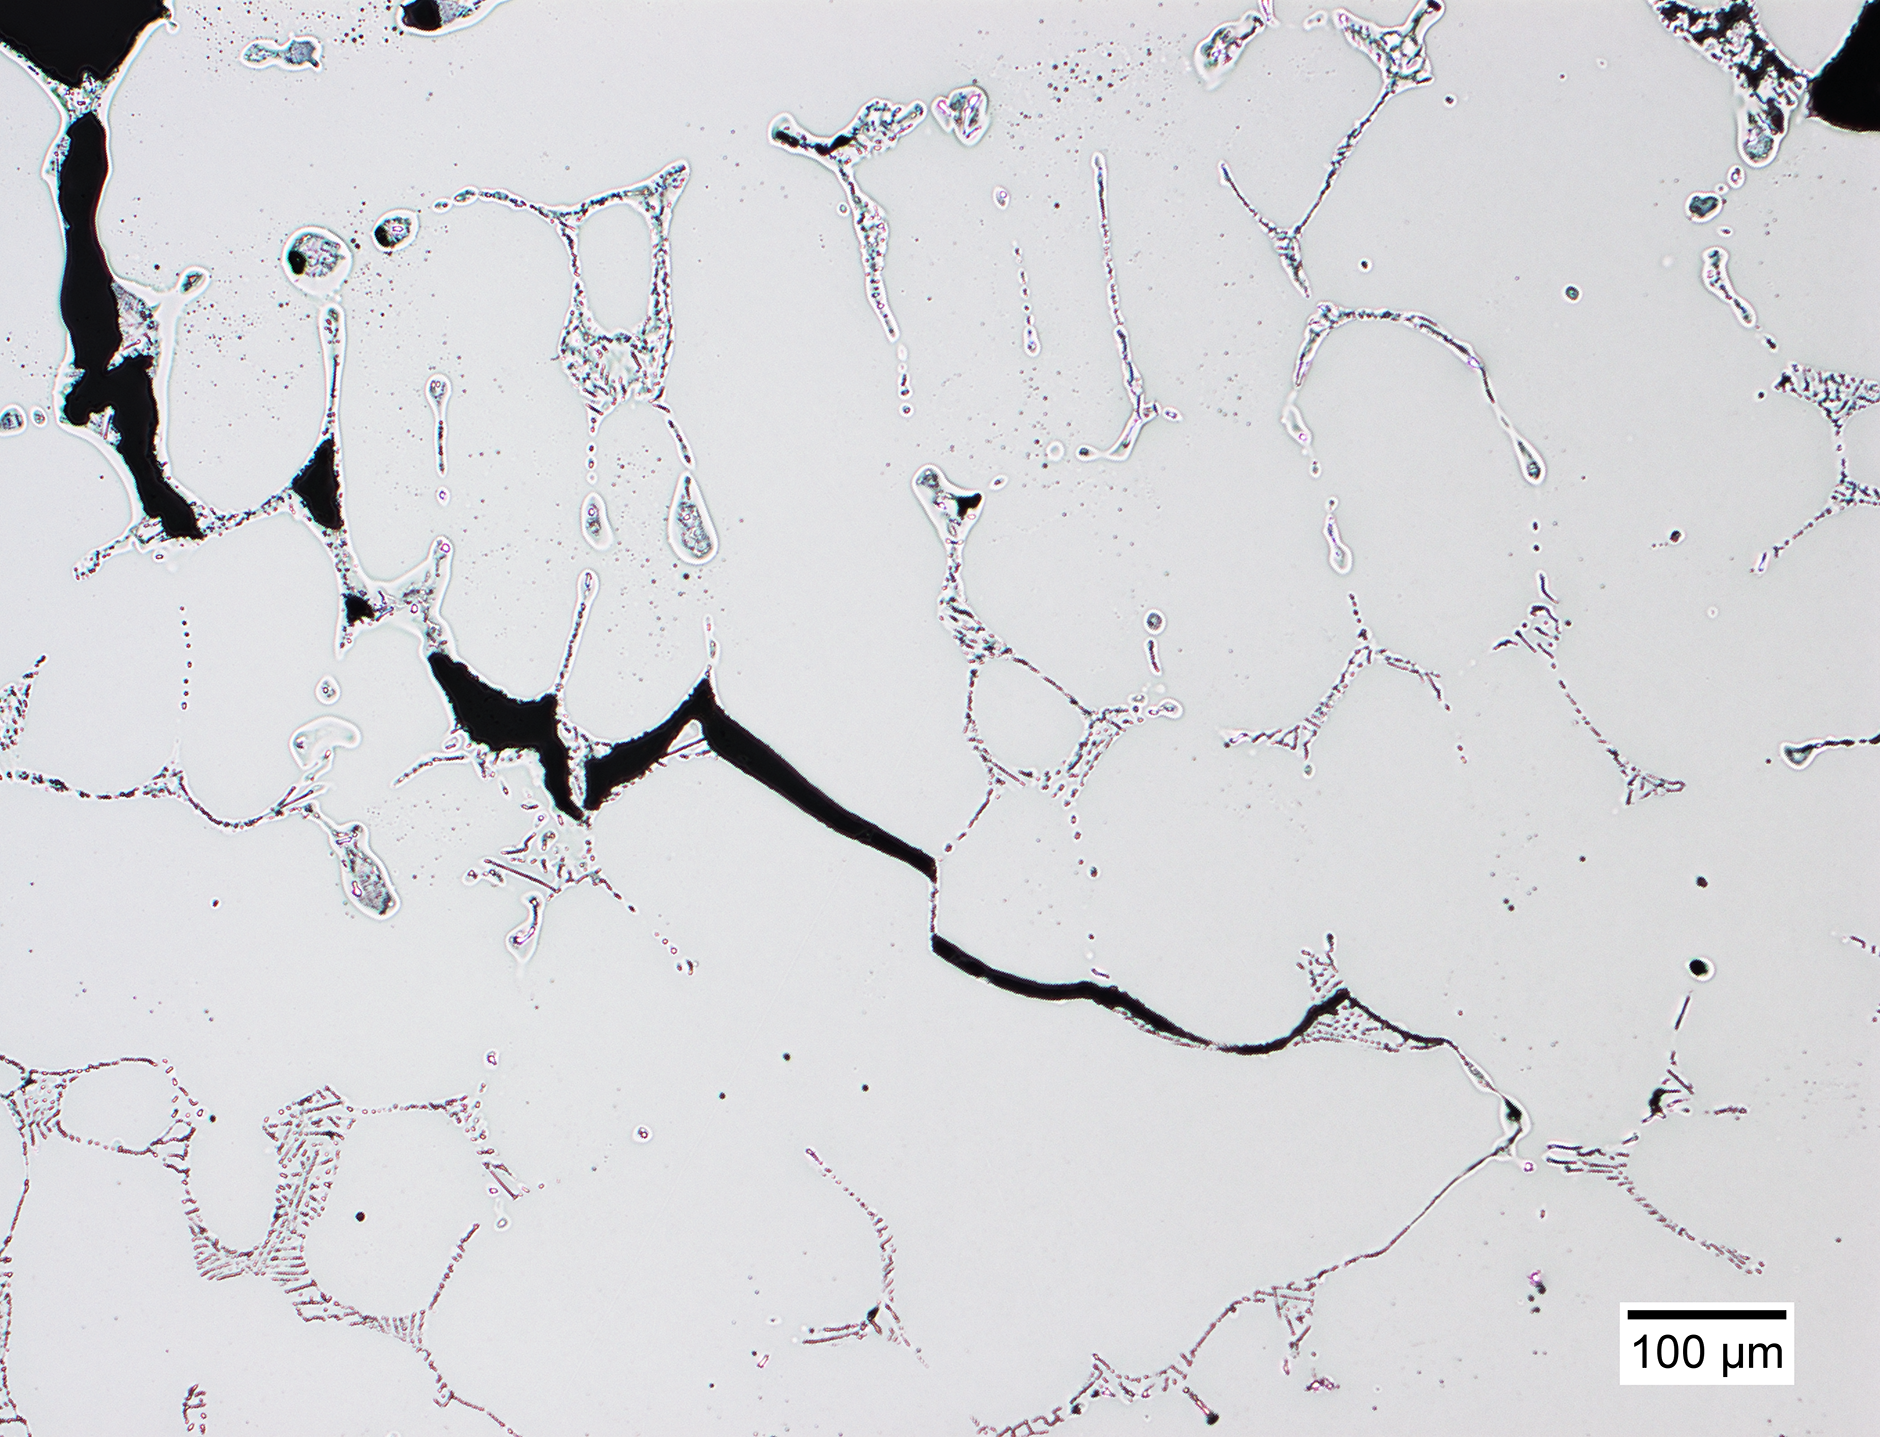
\includegraphics[width=4.7in]{figures/metallography/c5-oc-2300-crack-100x.png}} \\
    \subfloat[500X]{\label{subfig:c5-oc-2300-crack-500x}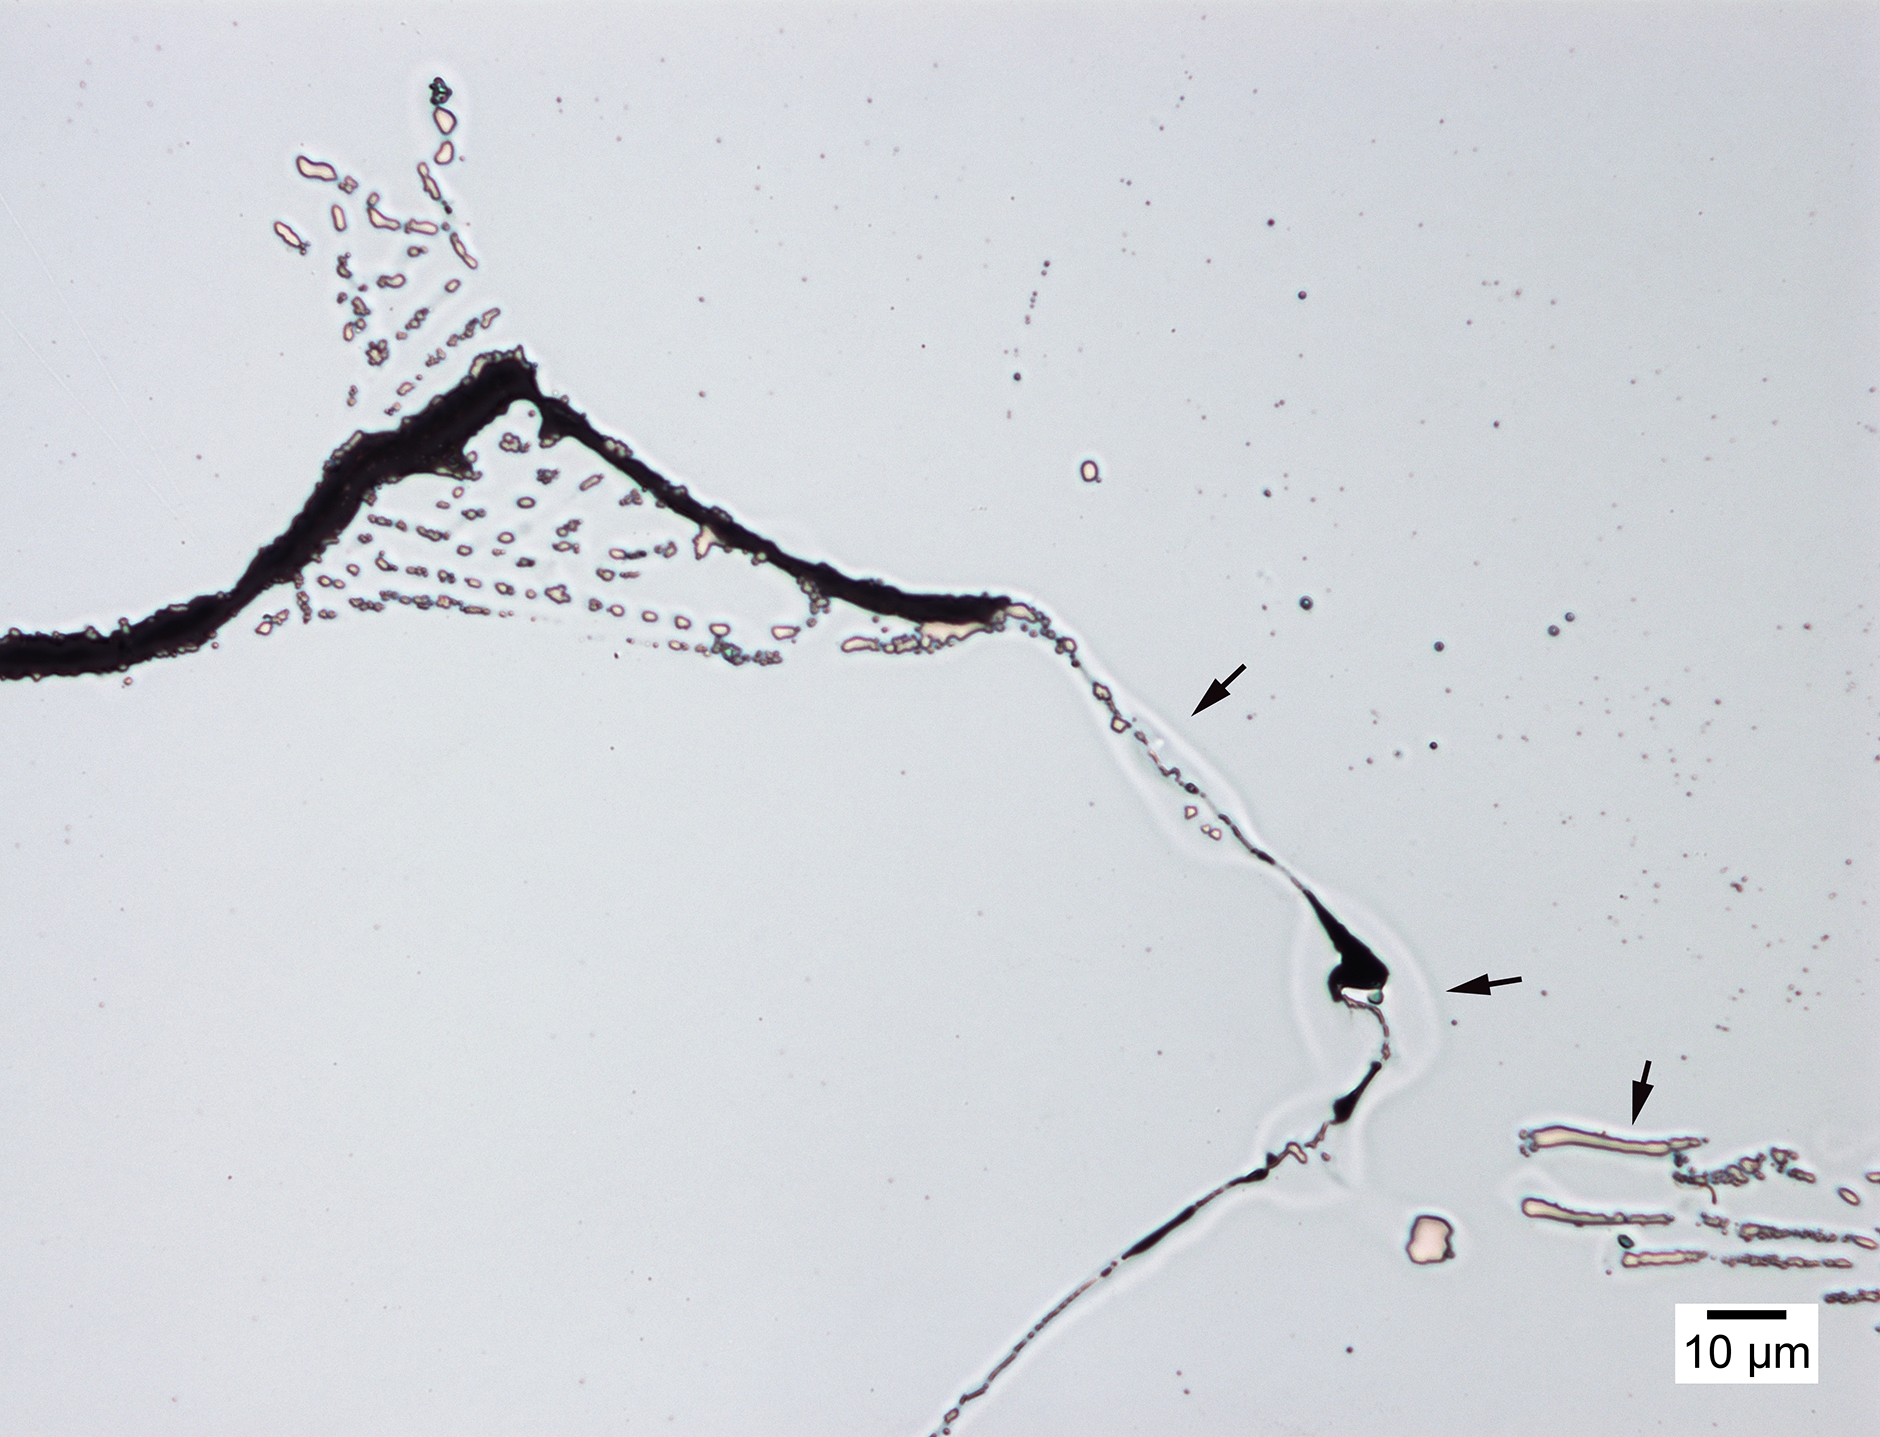
\includegraphics[width=4.7in]{figures/metallography/c5-oc-2300-crack-tip-500x.png}}
    \caption{Optical micrographs showing the crack visible in Figure~\ref{fig:c5-oc-2300-fracture-50x} for the Cone~5 On-Cooling 2300\textdegree{}F (C5 OC-2300) hot ductility sample. Liquated regions around the crack tip and interdendritic phases are denoted by arrows. Etch: electrolytic 10\% oxalic acid.}
    \label{fig:c5-oc-2300-crack-olm}
\end{figure}

\begin{figure}
    \centering
    \subfloat[1000X]{\label{subfig:c5-oc-2300-crack-sem-1kx}\includegraphics[width=4.7in]{figures/metallography/c5-oc-2300-crack-sem-1kx-L2-21.png}} \\
    \subfloat[5000X]{\label{subfig:c5-oc-2300-crack-sem-5kx}\includegraphics[width=4.7in]{figures/metallography/c5-oc-2300-crack-sem-5kx-L2-20.png}}
    \caption{\Gls{sem} micrographs of a crack tip region (cf. Figure~\ref{fig:c5-oc-2300-crack-olm}) in the Cone~5 On-Cooling 2300\textdegree{}F (C5 OC-2300) hot ductility sample. The \gls{eds} results for the indicated points ``A'' and ``B'' are given in Figure~\ref{fig:c5-oc-2300-crack-tip-eds}. Etch: electrolytic 10\% oxalic acid.}
    \label{fig:c5-oc-2300-crack-tip-sem}
\end{figure}

\begin{figure}
    \centering
    \subfloat[Spot \Gls{eds} results for point ``A'']{\label{subfig:c5-oc-2300-crack-eds-A}\includegraphics[width=\textwidth]{figures/metallography/c5-oc-2300-crack-eds-table-A.png}} \\
    \subfloat[Spot \Gls{eds} results for point ``B'']{\label{subfig:c5-oc-2300-crack-eds-B}\includegraphics[width=\textwidth]{figures/metallography/c5-oc-2300-crack-eds-table-B.png}}
    \caption{Spot \gls{eds} results for indicated points ``A'' and ``B'' in Figure~\ref{fig:c5-oc-2300-crack-tip-sem} at a crack tip region in the Cone~5 On-Cooling 2300\textdegree{}F (C5 OC-2300) hot ductility sample.}
    \label{fig:c5-oc-2300-crack-tip-eds}
\end{figure}


\begin{figure}
    \centering
    \subfloat[100X]{\label{subfig:c5-oc-2300-liquation-100x}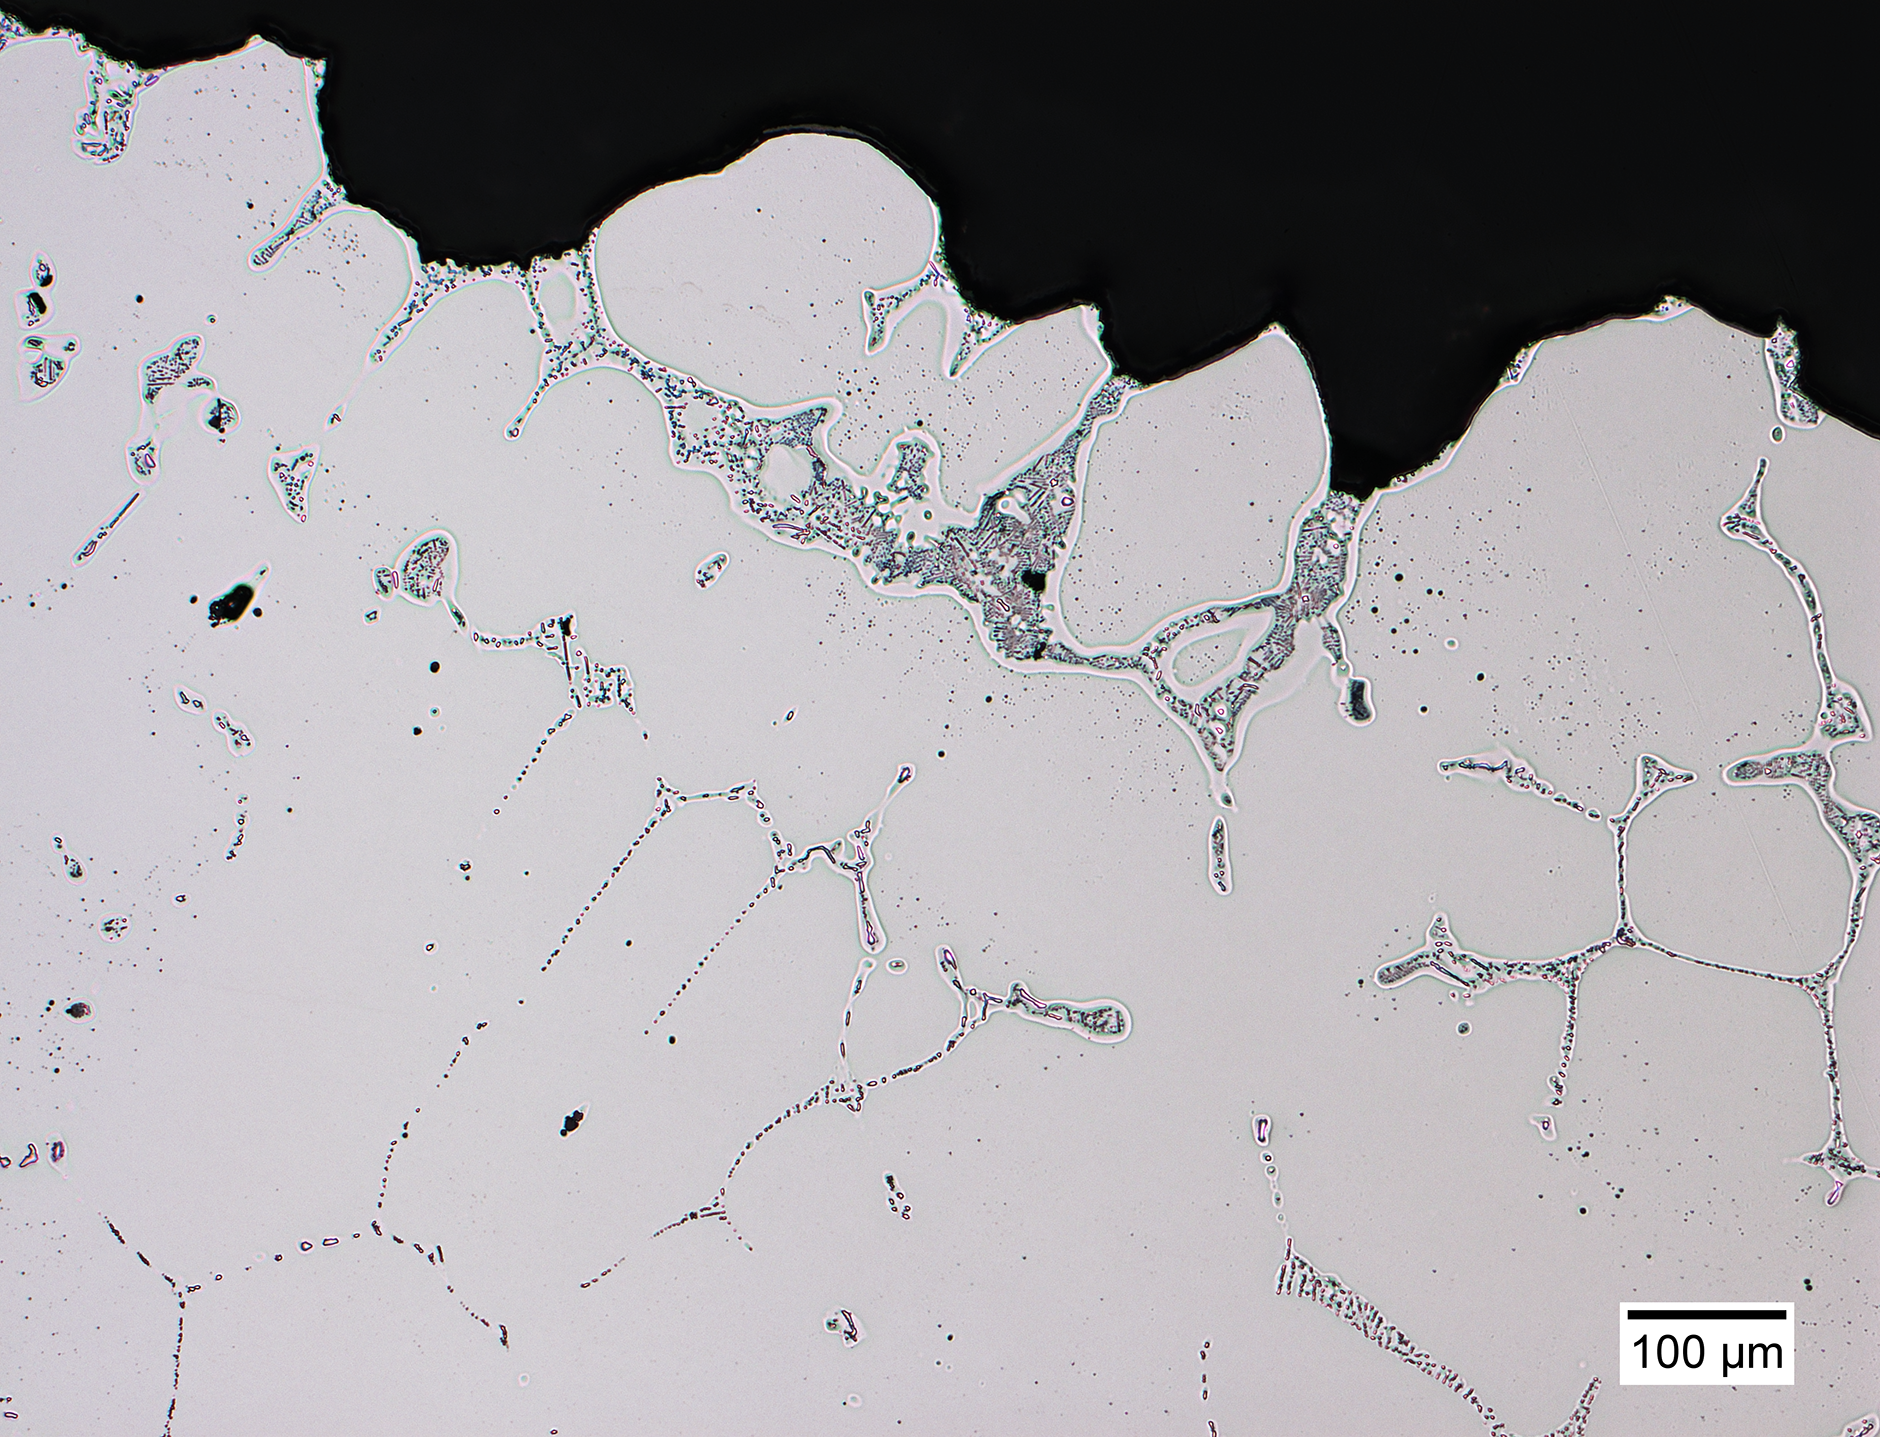
\includegraphics[width=4.7in]{figures/metallography/c5-oc-2300-liquation-100x.png}} \\
    \subfloat[500X]{\label{subfig:c5-oc-2300-liquation-500x}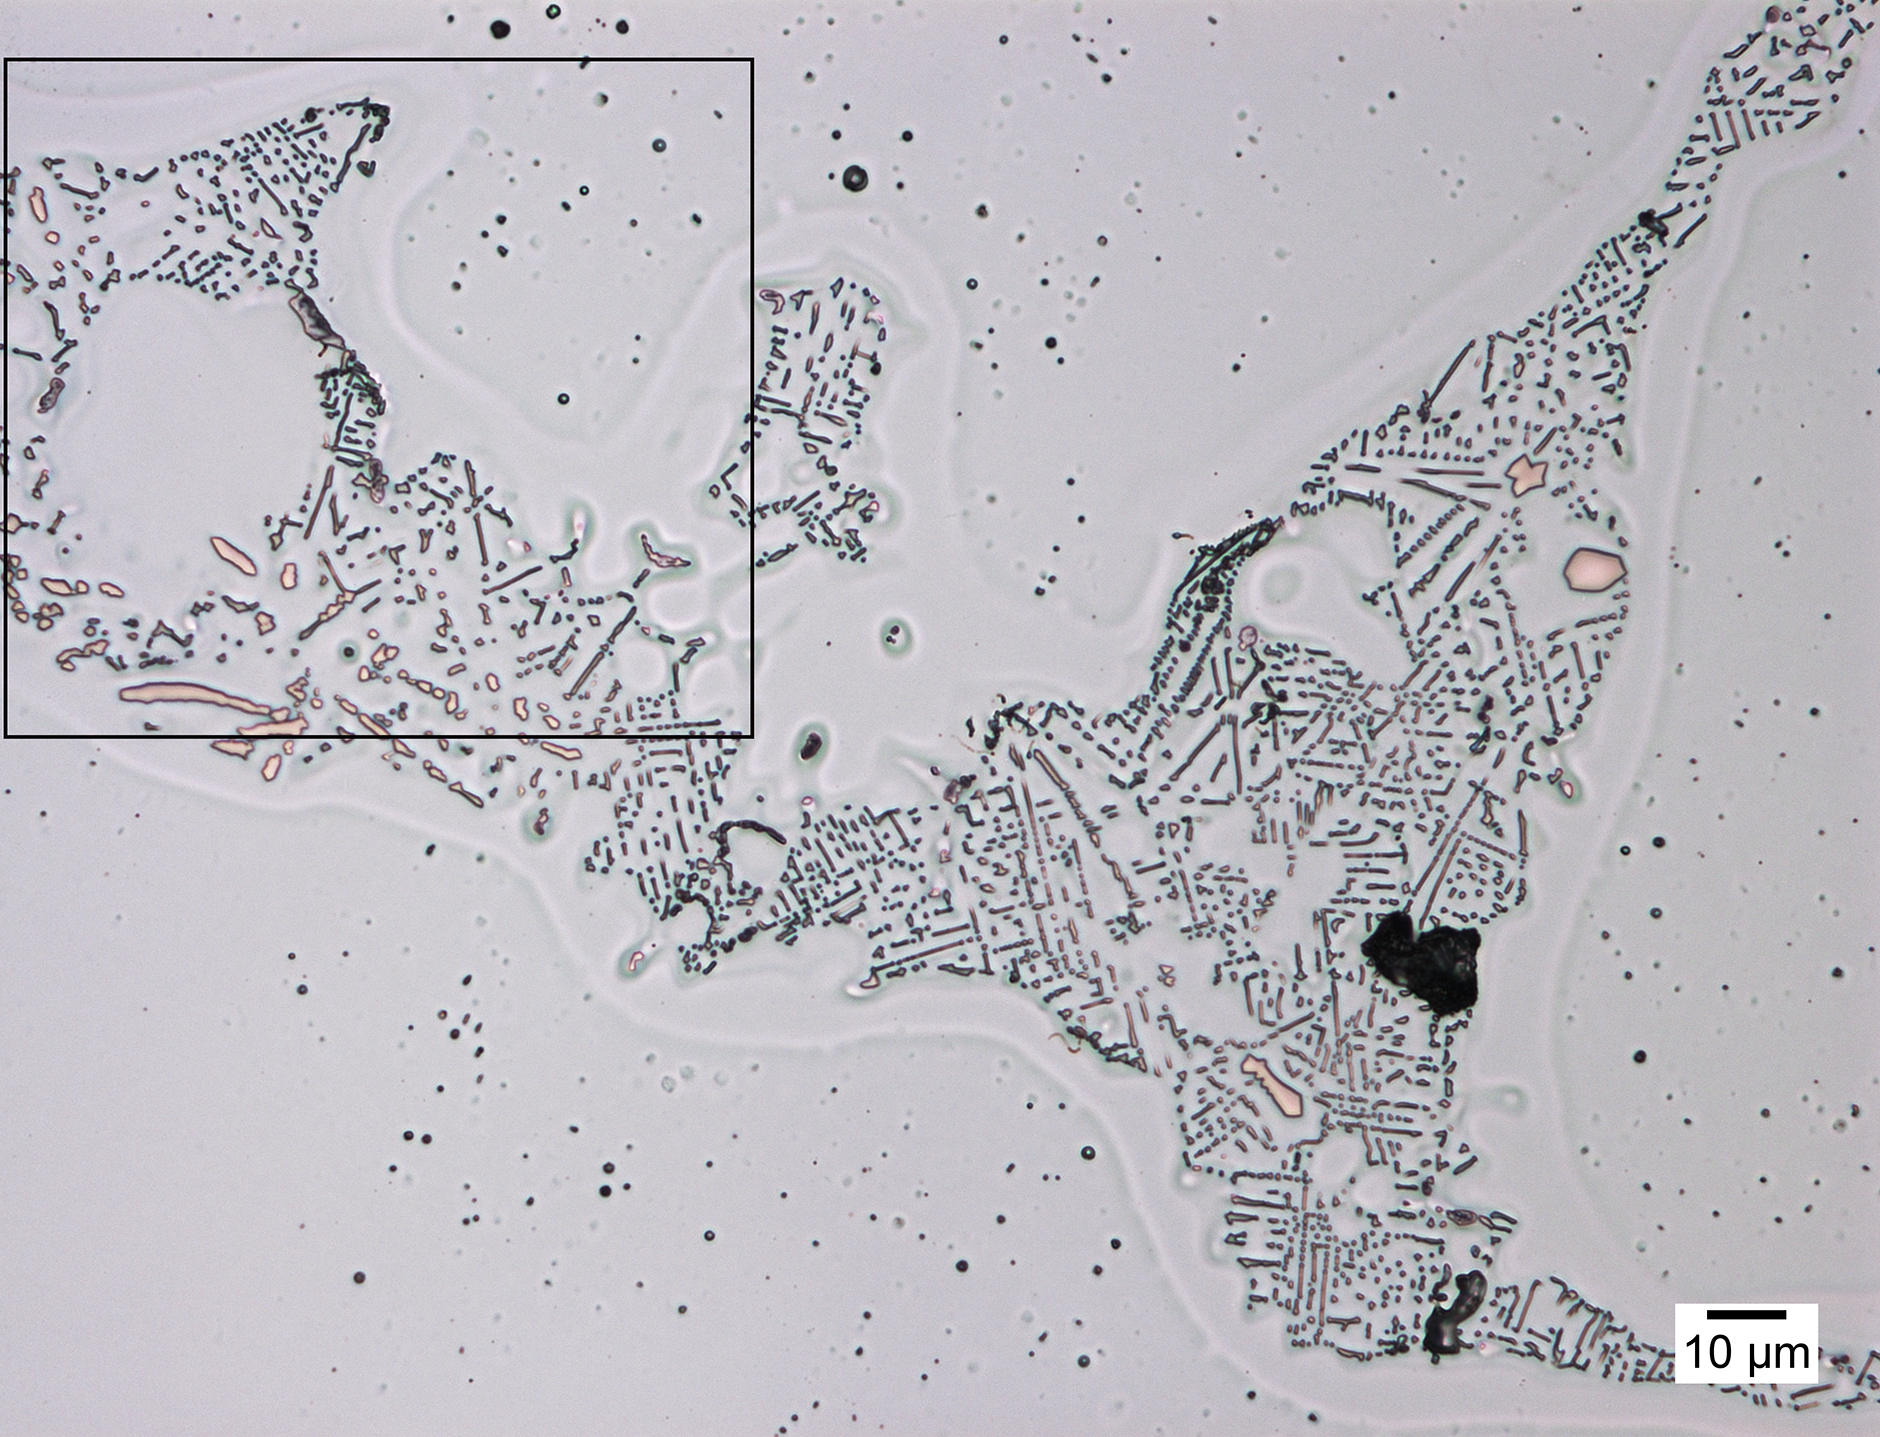
\includegraphics[width=4.7in]{figures/metallography/c5-oc-2300-liquation-500x.png}}
    \caption{Optical micrographs showing a liquated region adjacent to the fracture surface in the Cone~5 On-Cooling 2300\textdegree{}F (C5 OC-2300) hot ductility sample. The boxed region in (b) is examined at higher magnification in Figure~\ref{fig:c5-oc-2300-liquation-sem}. Etch: electrolytic 10\% oxalic acid.}
    \label{fig:c5-oc-2300-liquation-olm}
\end{figure}

\begin{figure}
    \centering
    \subfloat[2500X]{\label{subfig:c5-oc-2300-liquation-sem-2-5kx}\includegraphics[width=4.7in]{figures/metallography/c5-oc-2300-liquation-sem-2-5kx-L4-46.png}} \\
    \subfloat[5000X]{\label{subfig:c5-oc-2300-liquation-sem-5kx}\includegraphics[width=4.7in]{figures/metallography/c5-oc-2300-liquation-sem-5kx-L4-37.png}}
    \caption{\glsentryshort{bse}-\gls{sem} micrographs of the boxed region from Figure~\ref{fig:c5-oc-2300-liquation-olm} showing liquation surrounding interdendritic phases in the Cone~5 On-Cooling 2300\textdegree{}F (C5 OC-2300) hot ductility sample. \gls{eds} results for the three indicated points in (b) are given in Figure~\ref{fig:c5-oc-2300-liquation-eds}. Etch: electrolytic 10\% oxalic acid.}
    \label{fig:c5-oc-2300-liquation-sem}
\end{figure}

\begin{figure}
    \centering
    \subfloat[Spot \Glsentryshort{eds} results for point ``A'' corresponding to liquid in Figure~\ref{subfig:c5-oc-2300-liquation-sem-5kx}]{\label{subfig:c5-oc-2300-liquation-eds-table-A}\includegraphics[width=5.5in]{figures/metallography/c5-oc-2300-liquation-eds-table-A.png}} \\
    \subfloat[Spot \Gls{eds} results for point ``B'']{\label{subfig:c5-oc-2300-liquation-eds-table-B}\includegraphics[width=5.5in]{figures/metallography/c5-oc-2300-liquation-eds-table-B.png}} \\
    \subfloat[Spot \Gls{eds} results for point ``C'']{\label{subfig:c5-oc-2300-liquation-eds-table-C}\includegraphics[width=5.5in]{figures/metallography/c5-oc-2300-liquation-eds-table-C.png}}
    \caption{Spot \gls{eds} results for indicated points ``A'', ``B'', and ``C'' in Figure~\ref{fig:c5-oc-2300-liquation-sem} at a liquated region in the Cone~5 On-Cooling 2300\textdegree{}F (C5 OC-2300) hot ductility sample.}
    \label{fig:c5-oc-2300-liquation-eds}
\end{figure}